% mainfile: ../../Refinement.tex
In this section we investigate the trace semantics and some of its properties for gaining results for the refinement defined in \refSec{sec_de_sem_trace_ref}. Furthermore, these properties help in understanding the trace semantics and its applicability. Especially, we examine its behavior while applying a substitution and its relationship to simulation and bisimulation to classify the new semantics in the established context. The main part takes the investigation, whether the trace semantics is compositional or not, resulting by the fact that already the subclass of recursion-free processes is indeed not compositional for every operator.

As a first result we achieve that every set of traces is at most countably infinite. This is because we know that every trace is produced out of a countably infinite set of symbols. In other words, traces are words over a countably infinite alphabet. More precisely, for every $P\in\procs$ we know $\traces[P]\subseteq\left(\names\cup\conames\cup\mathtt{SYMB}\right)^*$ where $\mathtt{SYMB}$ denotes the set containing the angle brackets, the parenthesis, and the comma. Furthermore, we know that the countably infinite sets are closed under union and Kleene star. So, since $\names$ and $\conames$ are countably infinite, we know that the set $\traces[P]$ is countably infinite. Hence, we can define a function $\mathcal{T_I}:\procs_\alpha\rightarrow\pom{\N\times\tr}$, named \findex{indexed trace set}, such that every trace in the trace set of a equivalence class of a process is uniquely mapped to a natural number.

Furthermore, we know that every trace set $\traces[P]$ for a process $P\in\procs$ is closed under the prefix operator. Therefore, consider $s\in\traces[P]$. We know for every prefix $t\in\pref{\set{s}}$ that there is a trace $u\in\tr$ such that $s=\seqconc{t}{u}$. So there is a process $Q\in\procs$ such that $\ec{P}\bigstep{\seqconc{t}{u}}\ec{Q}$ and so $\ec{P}\bigstep{t}\fatsemi\bigstep{u}\ec{Q}$ holds. Hence, there is a process $Q'\in\procs$ such that $\ec{P}\bigstep{t}\ec{Q'}$ and so $t\in\traces[P]$.

Since the empty sequence is a prefix of every trace, it fits that the empty trace is included in every trace set.

\begin{lemma}[Empty trace]
\label{lem_empty_trace}
For all $P\in\procs$
\[\eseq\in\traces[P]\]
holds.
\end{lemma}
\begin{prf}
Let $P\in\procs$. Since $\left(\tautrans\right)^*$ is reflexive, we know that $\ec{P}\left(\tautrans\right)^*\ec{P}$ holds. With the definition of the big-step semantics (\refDef{def_bigstep_semantics}) we get $\ec{P}\bigstep{\eseq}\ec{P}$. With that and from the definition of the trace semantics (\refDef{def_trace_semantics}) we know that $\eseq\in\traces[P]$ holds, since $P\in\procs$.
%%%%%%%%%%%%%%%%%%%%%%%%%%%%%%%%%%%%%%%%%%%%%% START LONG VERSION %%%%%%%%%%%%%%%%%%%%%%%%%%%%%%%%%%%%%%%%%%%%%%%%%%%%%%%%%%%%%%%%%%%%%%%%%%%%%%
\begin{old}{long version}
	Let $P\in\procs$. With the definition of the trace semantics (\refDef{def_trace_semantics}), we know that
		\[\traces[P] = \set[\exists{}Q\in\procs:\ec{P}\bigstep{t}\ec{Q}]{t\in\tr}\]
	holds. Since $P\in\procs$ we have
	\[\traces[P]=\underbrace{\set[\ec{P}\bigstep{t}\ec{P}]{t\in\traces}}_{Y\define} \cup \set[\exists{}Q\in\procs: Q\nin\ec{P} \wedge\ec{P}\bigstep{t}\ec{Q}]{t\in\tr}.\]
	We know from the definition of the big-step semantics (\refDef{def_bigstep_semantics}) that $\ec{P}\bigstep{\eseq}\ec{P}$ if and only if $\ec{P}\left(\tautrans\right)^*\ec{P}$. Since $\left(\tautrans\right)^*$ is a reflexive and transitive closure, we know that $\ec{P}\left(\tautrans\right)^*\ec{P}$ holds, which means $\ec{P}\bigstep{\eseq}\ec{P}$ holds, and therefore $\eseq{}\in{}Y$ and so $\eseq\in\traces[P]$.
\end{old}
%%%%%%%%%%%%%%%%%%%%%%%%%%%%%%%%%%%%%%%%%%%%%% END LONG VERSION %%%%%%%%%%%%%%%%%%%%%%%%%%%%%%%%%%%%%%%%%%%%%%%%%%%%%%%%%%%%%%%%%%%%%%%%%%%%%%
\end{prf}

Now, we examine the behavior of the trace semantics in the context of substitutions.

\subsection{Substitution}
\label{sec_de_sem_trace_prop_subst}
% mainfile: ../../Refinement.tex
%Since we proved in \refLem{lem_subst_bigstep_partII} that if we have a trace between two processes, we also can apply a substitution on the processes and the trace, and the big-step stays preserved, we can directly lift this statement upon the trace semantics.
Due to \refLem{lem_subst_bigstep_partII}, traces between two processes are preserved under substitution. We can lift this result to the trace semantics.
\begin{lemma}[Substitution on trace semantics (Part I)]
\label{lem_subst_trace_partI}
	For all $P\in\procs$ and substitutions $\sigma$ 
		\[\traces[P]\sigma\subseteq\traces[P\sigma]\]
	holds.
\end{lemma}
\begin{prf}
Let $P\in\procs$, $\sigma$ a substitution, and $s\in\left(\traces[P]\sigma\right)$. Then we know from the definition of the substitution on traces and the trace semantics that there exists a process $Q\in\procs$ and a trace $s'\in\tr$ such that $\ec{P}\bigstep{s'}\ec{Q}$ and $s=s'\sigma$ holds. \refLem{lem_subst_bigstep_partII} yields that $\ec{P\sigma}\bigstep{s'\sigma}\ec{Q\sigma}$ holds. So we know $\ec{P\sigma}\bigstep{s}\ec{Q\sigma}$ and since $Q\sigma\in\procs$, we know from the definition of the trace semantics that $s\in\traces[P\sigma]$.
\end{prf}

From the example to \refLem{lem_subst_bigstep_partII} we already know that the converse set inclusion does not hold. Because there, we found a trace $\seq{\out{y}{c}}\in\traces[P\subs{a}{b}]$ for $P\define\procpar{\inp{a}{x}.\out{x}{c}}{\out{b}{y}.\out{c}{d}}$ and argued that no trace $s$ starting in $\ec{P}$ can satisfy $s\sigma=\seq{\out{y}{c}}$. So $\seq{\out{y}{c}}\nin\traces[P]\sigma$.

But once more, we can prove a restricted version of the converse of the previous Lemma and this directly leads to a restricted version of a set equality.

\begin{lemma}[Substitution on trace semantics (Part II)]
\label{lem_subst_trace_partII}
Given $a,b\in\names$, $P\in\procs$ then
\[\traces[P\transp{a}{b}]=\traces[P]\transp{a}{b}\]
holds.
\end{lemma}
\begin{prf}
Let $a,b\in\names$, $P\in\procs$ and $\sigma=\transp{a}{b}$ transposition. Then, \refLem{lem_subst_trace_partI} directly yields $\traces[P\transp{a}{b}]\supseteq\traces[P]\transp{a}{b}$ since a transposition is a special case of a substitution. For the other inclusion we take a trace $s'\in\traces[P\sigma]$. Thus, there is a process $Q'\in\procs$ such that $\ec{P\sigma}\bigstep{s'}\ec{Q'}$. \refLem{lem_subst_bigstep_partIV} yields that there is a process $Q\in\procs$ and a trace $s\in\tr$ with $\ec{P}\bigstep{s}\ec{Q}$ and $s\transp{a}{b}=s'$. Hence, $s\in\traces[P]$ and so $s'\in\traces[P]\transp{a}{b}$.
\end{prf}

Thus, for a transposition the trace sets are equal no matter whether the transposition is applied to the process or to the trace set. Furthermore, for a substitution which only replaces one name which is a fresh one for the process, the trace set of the process with applied substitution is the same as the trace set of the process where a transposition of the names of the substitution is applied to every trace. This is because of $\ec{P\sigma}=\ec{P\transp{a}{b}}$ for a substitution $\sigma\define{}\subs{a}{b}$ and $a\nin\fn{P}$.

Furthermore, we can see that the set inclusion is preserved under the application of a substitution.

\begin{lemma}[Substitution and trace inclusion (Part I)]
\label{lem_subst_trace_inclusion}
For all processes\newline{}$P,Q\in\procs$ and substitutions $\sigma$,
\[\text{if }\traces[P]\subseteq\traces[Q] \text{ then } \traces[P]\sigma\subseteq\traces[Q]\sigma\]
holds.
\end{lemma}
\begin{prf}
Let $P,Q\in\procs$, $\sigma$ a substitution, and $\traces[P]\subseteq\traces[Q]$. Given $s\in\traces[P]\sigma$, we know there has to be a trace $s'\in\traces[P]$, with $s=s'\sigma$. So $s'\in\traces[Q]$ holds and also $s=s'\sigma\in\traces[Q]\sigma$ holds.
\end{prf}

The converse of the previous lemma cannot hold. Consider, for example, $P\define{}\out{a}{x}$, $Q\define{}\out{b}{x}$ and $\sigma\define\subs{a}{b}$. Then $\traces[P]=\set{\eseq,\seq{\outa{a}{x}}}$, and $\traces[Q]=\set{\eseq,\seq{\outa{b}{x}}}$. Hence, $\traces[P]\sigma=\set{\eseq,\seq{\outa{a}{x}}}$ and $\traces[Q]\sigma=\set{\eseq,\seq{\outa{a}{x}}}$. Thus, $\traces[P]\sigma\subseteq\traces[Q]\sigma$ but $\traces[P]\not\subseteq{}\traces[Q]$.

In spite of that, \refLem{lem_subst_trace_partII} and \refLem{lem_subst_trace_inclusion} yield directly a helpful connection between trace set inclusion and a transposition.

\begin{cor}[Substitution and trace inclusion (Part II)]
\label{cor_subst_trace_inclusion}
Given $P,Q\in\procs$ and $a,b\in\names$ then,
\[\text{if }\traces[P]\subseteq\traces[Q] \text{ then } \traces[P\transp{a}{b}]\subseteq\traces[Q\transp{a}{b}]\]
holds
\end{cor}
\begin{prf}
Let $P,Q\in\procs$ and $\sigma=\transp{a}{b}$ be a transposition with $\traces[P]\subseteq\traces[Q]$. Furthermore, let $t\in\traces[P\sigma]$. On the one hand \refLem{lem_subst_trace_partII} yields that $t\in\traces[P]\transp{a}{b}$ and on the other hand \refLem{lem_subst_trace_inclusion} yields that $\traces[P]\transp{a}{b}\subseteq\traces[Q]\transp{a}{b}$. Thus, $t\in\traces[Q]\transp{a}{b}$ and again with \refLem{lem_subst_trace_partII} we know $t\in\traces[Q\sigma]$ holds.
\end{prf}

Thus, for transpositions, the trace inclusion is preserved. Furthermore, since $\ec{P\sigma}=\ec{P\transp{a}{b}}$ for a substitution $\sigma\define{}\subs{a}{b}$ and $a\nin\fn{P}$, we know \refCor{cor_subst_trace_inclusion} is also true for a substitution which only replaces one name with a new fresh one.


\subsection{Compositionality}
\label{sec_de_sem_trace_prop_comp}
% mainfile: ../../Refinement.tex
In this section we investigate the compositionality of the trace semantics. That is, for a binary operator $\circ$ on processes, we have a binary operation $\circ{}_{\mathcal T}$ on the trace sets such that $\traces[P\circ{}Q]=\traces[P]\circ{}_{\mathcal T}\traces[Q]$ holds. By this investigation, we get that a formal compositionality of every operator most likely does not exist. For example, consider an input process $\inp{a}{x}.P$, then the new communications, which can be established by the incoming name, can possibly not be obtained by the traces of $P$. Therefore, we develop a algorithmic notion for calculating a subset of the traces compositional. That is, we can algorithmically calculate the traces of a process compositional, if we assume that only a finite number of names can be send from the outside to the process.
%\todo{also guess otherwise not possible}

Furthermore, we restrict the compositionality of the parallel operator to the class of restriction-free and recursion-free processes for reasons of simplicity. This is of minor influence, since we know with \refLem{lem_extended_standard_form} that every process can be transformed in extended standard form such that all restriction operators are right at the front of the process. Additionally, by a suitable unfolding technique of the process calls, we assume that we can possibly get rid of the restriction to recursion-free process as long as we can find some kind of fix-point algorithm for the unfolding. However, this investigation was out of the scope of this thesis. For practically usage of this semantics, the following results appear to be helpful.

\subsubsection{Inaction, $\tau$ and output process, choice}
We start the investigation of the compositionality of the trace semantics with the unproblematic cases for the inaction, the $\tau$ and output process, and the choice.

\begin{lemma}[Compositionality: $\tau$ processes/output processes/choices]
\label{lem_compositionality_traces}
Given processes $P,Q\in\procs$ and names $a,x\in\names$, then
	\begin{align*}
		\traces[\proczero] &= \set{\eseq} \tag{INACTION}\label{eq_compo_inaction}\\
		\traces[\tau.P] &= \traces[P] \tag{TAU}\label{eq_compo_tau}\\
		\traces[\out{a}{x}.P] &= \set{\eseq}\cup\seqconc{\set{\seq{\outa{a}{x}}}}{\traces[P]} \tag{OUTPUT}\label{eq_compo_output}\\%\set[{s\in\traces[P]}]{\seqconc{\seq{\out{a}{x}}}{s}}
		\traces[\procchoice{P}{Q}] &= \traces[P] \cup \traces[Q]	\tag{CHOICE}\label{eq_compo_choice}\\
		%\traces[\proccall{A}{\vec{v}}] &= \traces[P\subs{\vec{v}}{\vec{w}}] \text{ with } \procdef{A}{\vec{w}}\define{}P\tag{CALL}\label{eq_compo_call}
	\end{align*}
holds.
%\item \todo{Für parallel reicht nicht. Problem: zuviel Verhalten bei gebundenem Output}Let $T_P\define\set[\nexists\bout{a}{x}\in{}s:x\in\fn{Q}]{s\in\traces[P]}$ and \newline
%$T_Q\define\set[\nexists\bout{a}{x}\in{}s:x\in\fn{P}]{s\in\traces[Q]}$, then
%			\begin{align*}
%			\traces[\procpar{P}{Q}] = \bigcup_{(s,t)\in{}T_P\times{}T_Q}{s\seqcom{}t}.
%			\end{align*}
			%%%%%%%%%%%%%%%%%%%%%%%%%%%%%%%%%%%%%%%%%%%%% THIRD VERSION %%%%%%%%%%%%%%%%%%%%%%%%%%%%%%%%%%%%%%%%%%%%%%%%%%%%%%%%%%%%%%%%%%%%%%%%%%%%%%%%%%
%		\item Let $T_B\define\bind{a}{\traces[P]}$ and with that \newline$T_P\define{}T_B\setminus\bigl(\left\{s\in{}T_B \; \mid \; \exists{}i,j\in\N:a\in\sub{s_i}\wedge{}a\in\obj{s_j}\wedge{}i\leq{}j\right\}$\newline{} $\cup \set[\exists{}i\in\N\nexists{}j\in\N:a\in\sub{s_i}\wedge{}a\in{}\obj{s_j}]{s\in{}T_B}\bigr)$, then
%\set[\exists{}i,j\in\N:a\in\sub{s_i}\wedge{}a\in\obj{s_j}\wedge{}i\leq{}j]{s\in{}T_B}
%			\[\traces[\procres{a}{P}] = \bigcup_{a'\in\names}\left(T_P\subs{a'}{a}\right)\]			
			%%%%%%%%%%%%%%%%%%%%%%%%%%%%%%%%%%%%%%%%%%%%% SECOND VERSION %%%%%%%%%%%%%%%%%%%%%%%%%%%%%%%%%%%%%%%%%%%%%%%%%%%%%%%%%%%%%%%%%%%%%%%%%%%%%%
			\begin{old}{second version}		
				Let $T_P\define\traces[P]\setminus\bigl(\set[a\in_c s]{s\in\traces[P]}\cup\set[\out{b}{a}\in s,b\in\names]{s\in\traces[P]}\bigr)\cup \set[{s\in\traces[P]}]{s\subs{\left(a\right)}{\langle{}a\rangle}}$, then
					\[\traces[\procres{a}{P}] = \bigcup_{a'\in\names}\left(T_P\subs{a'}{a}\right)\]
			\end{old}
			%%%%%%%%%%%%%%%%%%%%%%%%%%%%%%%%%%%%%%%%%%%%%% END SECOND VERSION %%%%%%%%%%%%%%%%%%%%%%%%%%%%%%%%%%%%%%%%%%%%%%%%%%%%%%%%%%%%%%%%%%%%%%%%%%%%%%
			%%%%%%%%%%%%%%%%%%%%%%%%%%%%%%%%%%%%%%%%%%%%% FIRST VERSION %%%%%%%%%%%%%%%%%%%%%%%%%%%%%%%%%%%%%%%%%%%%%%%%%%%%%%%%%%%%%%%%%%%%%%%%%%%%%%
			\begin{old}{first version}		
				\begin{align*}
				\traces[\procres{a}{P}] = \bigcup_{a'\in\names}\bigl(\traces[P]\subs{a'}{a}&\setminus\bigl(\set[a'\in_c s]{s\in\traces[P]\subs{a'}{a}} \\
							& \quad\quad\cup \set[\outa{b}{a'}\in s,b\in\names]{s\in\traces[P]\subs{a'}{a}}\bigr) \\
							&\cup \set[{s\in\traces[P]\subs{a'}{a}}]{s\subs{\left(a'\right)}{\langle{}a'\rangle}}\bigr).
				\end{align*}
			\end{old}
			%%%%%%%%%%%%%%%%%%%%%%%%%%%%%%%%%%%%%%%%%%%%%% END FIRST VERSION %%%%%%%%%%%%%%%%%%%%%%%%%%%%%%%%%%%%%%%%%%%%%%%%%%%%%%%%%%%%%%%%%%%%%%%%%%%%%%
\end{lemma}
\begin{prf}
To prove \refLem{lem_compositionality_traces} we handle every case individually.
\begin{description}
%%%%%%%%%%%%%%%%%%%%%%%%%%%%%%%%%%%%%%%%%%%%%%%%%%%%%%%%%% ZERO %%%%%%%%%%%%%%%%%%%%%%%%%%%%%%%%%%%%%%%%%%%%%%%%%%%%%%%%%%%%%%%%%%%%%%%%%%%%%%%%%%%%%%%%%%%%%%%%%%%%%%%%%%%
\item[Case {$\traces[\proczero]$}:]
From the definition of the trace semantics (\refDef{def_trace_semantics}) we know that
\begin{align*}
\label{eq_trace_proc_zero}
	\traces[\proczero] = \set[\exists{}Q\in\procs:\ec{\proczero}\bigstep{t}\ec{Q}]{t\in\tr}
\end{align*}
holds. Furthermore, with \refLem{lem_empty_trace} we know $\eseq\in\traces[\proczero]$ so that
\begin{align}
\label{eq_trace_proc_zero}
	\traces[\proczero] = \set{\eseq{}}\cup \underbrace{\set[\exists{}Q\in\procs:\ec{\proczero}\bigstep{t}\ec{Q}]{t\in\tr\setminus\set{\eseq}}}_{Y\define{}}.
\end{align}
Let us assume that $Y\neq\emptyset$ and therefore let $t\in{}Y$. Then, from \refEq{eq_trace_proc_zero}, we know that a process $Q\in\procs$ must exist such that $\ec{\proczero}\bigstep{t}\ec{Q}$. Since $t\neq\eseq$, there has to be an action $\alpha\in{}t$ with $\alpha\neq\tau$ and a trace $s\in\tr$ due to the definition of the big-step semantics (\refDef{def_bigstep_semantics}) such that $\ec{\proczero}\bigstep{}\fatsemi\transs{\alpha}\fatsemi\bigstep{s}\ec{Q}$ holds and $t=\seqconc{\seq{\alpha}}{s}$. But there is no rule of the operational semantics (\refDef{def_early_trans_system}), such that for a process $Q'\in\procs$, there is a transition like $\ec{\proczero}\tautrans\ec{Q'}$ or $\ec{\proczero}\transs{\alpha}\ec{Q'}$. This is a contradiction, thus, $Y=\emptyset$. Hence with \refEq{eq_trace_proc_zero} we know that all in all 
\[\traces[\proczero]=\set{\eseq}\]
holds.
%%%%%%%%%%%%%%%%%%%%%%%%%%%%%%%%%%%%%%%%%%%%% START LONG VERSION %%%%%%%%%%%%%%%%%%%%%%%%%%%%%%%%%%%%%%%%%%%%%%%%%%%%%%%%%%%%%%%%%%%%%%%%%%%%%%
\begin{old}{long version}
	\begin{align*}
		\begin{array}{lcl}
		\traces[\proczero] &\eq{\text{def.}}& \set[\exists{}Q\in\procs:\ec{\proczero}\bigstep{t}\ec{Q}]{t\in\tr} \\
				&\eq{\proczero\in\procs}& \set{\eseq} \cup \set[\exists{}\proczero\neq{}Q\in\procs:\ec{\proczero}\bigstep{t}\ec{Q}\wedge{}t\neq\eseq]{t\in\tr}\\
				&\eq{}& \set{\eseq} \cup \bigl\{t\in\tr\;\mid\;\exists{}\proczero\neq{}Q\in\procs,\tau\neq\alpha\in{}t,s\in\tr:\\&&\quad\quad\quad\quad\quad\quad\quad\quad\quad\ec{\proczero}\bigstep{}\fatsemi\transs{\alpha}\fatsemi\bigstep{s}\ec{Q}\wedge{}t=\seqconc{\seq{\alpha}}{s}\bigr\}\\
				&\eq{(*)}& \set{\eseq} \cup \emptyset\\
				&\eq{}& \set{\eseq}
		\end{array}
	\end{align*}
$(*)$ No rule in \refFig{fig_ts_early} exists, such as for $Q\in\procs$ and $\alpha\in\actions$ there is a transition like $\ec{\proczero}\transs{\tau}\ec{Q}$ or $\ec{\proczero}\transs{\alpha}\ec{Q}$.
\end{old}
%%%%%%%%%%%%%%%%%%%%%%%%%%%%%%%%%%%%%%%%%%%%%% END LONG VERSION %%%%%%%%%%%%%%%%%%%%%%%%%%%%%%%%%%%%%%%%%%%%%%%%%%%%%%%%%%%%%%%%%%%%%%%%%%%%%%

%%%%%%%%%%%%%%%%%%%%%%%%%%%%%%%%%%%%%%%%%%%%%%%%%%%%%%%%%% TAU %%%%%%%%%%%%%%%%%%%%%%%%%%%%%%%%%%%%%%%%%%%%%%%%%%%%%%%%%%%%%%%%%%%%%%%%%%%%%%%%%%%%%%%%%%%%%%%%%%%%%%%%%%%
\item[Case {$\traces[\tau.P]$}:]
Let $P\in\procs$. As in the prior case we know from \refDef{def_trace_semantics} that
\begin{align*}
	\traces[\tau.P] = \set[\exists{}Q\in\procs:\ec{\tau.P}\bigstep{t}\ec{Q}]{t\in\tr}
\end{align*}
From the definition of the operational semantics (\refDef{def_early_trans_system}) we know that there is only one rule, which handles a $\tau$ prefix. Hence with the \etau{} rule we know that
	\[\traces[\tau.P] =\set[\exists{}Q\in\procs:\ec{\tau.P}\tautrans\ec{P}\wedge\ec{P}\bigstep{s}\ec{Q}\wedge t = \seqconc{\eseq}{s}]{t\in\tr}\]
holds, due to the fact that $\tau$ actions are omitted in traces. Since $\ec{\tau.P}\tautrans\ec{P}$ is true for all $P\in\procs$, it can be omitted so that
	\[\traces[\tau.P]=\set[\exists{}Q\in\procs:\ec{P}\bigstep{s}\ec{Q}\wedge t = \seqconc{\eseq}{s}]{t\in\tr}\]
holds. This leads with the definition of the concatenation of traces and the definition of the trace semantics to $\traces[\tau.P]=\traces[P]$.
%%%%%%%%%%%%%%%%%%%%%%%%%%%%%%%%%%%%%%%%%%%%% START SHORT VERSION %%%%%%%%%%%%%%%%%%%%%%%%%%%%%%%%%%%%%%%%%%%%%%%%%%%%%%%%%%%%%%%%%%%%%%%%%%%%%%
\begin{old}{short version}
	\begin{align*}
		\begin{array}{lcl}
			\traces[\tau.P] &\eq{\text{def.}}& \set[\exists{}Q\in\procs:\ec{\tau.P}\bigstep{t}\ec{Q}]{t\in\tr} \\
					&\eq{\tau.P\in\procs}& \set{\eseq} \cup \set[\exists{}\ec{\tau.P}\ni{}Q\in\procs:\ec{\tau.P}\bigstep{t}\ec{Q}]{t\in\tr}\\
					&\eq{\text{\etau}}& \set{\eseq}\cup \seqconc{\set{\eseq}}{\set[\exists{}Q\in\procs:\ec{P}\bigstep{t}\ec{Q}]{t\in\tr}}\\
					&\eq{\text{def.}}& \set{\eseq}\cup \seqconc{\set{\eseq}}{\traces[P]}\\
					&\eq{\text{def.}}& \set{\eseq}\cup \traces[P]\\
					&\eq{\text{ref}}& \traces[P]
		\end{array}
	\end{align*}	
\end{old}
%%%%%%%%%%%%%%%%%%%%%%%%%%%%%%%%%%%%%%%%%%%%% END SHORT VERSION %%%%%%%%%%%%%%%%%%%%%%%%%%%%%%%%%%%%%%%%%%%%%%%%%%%%%%%%%%%%%%%%%%%%%%%%%%%%%%
%%%%%%%%%%%%%%%%%%%%%%%%%%%%%%%%%%%%%%%%%%%%%%%%%%%%%%%%%% OUTPUT %%%%%%%%%%%%%%%%%%%%%%%%%%%%%%%%%%%%%%%%%%%%%%%%%%%%%%%%%%%%%%%%%%%%%%%%%%%%%%%%%%%%%%%%%%%%%%%%%%%%%%%%%%%
\item[Case {$\traces[\out{a}{x}.P]$}:]
Let $P\in\procs$ be a process and $a,x\in\names$ be names. From \refDef{def_trace_semantics} and \refLem{lem_empty_trace} we, analogously to the stop process case, know that
\begin{align}
\label{eq_trace_out}
	\traces[\out{a}{x}.P] = \set{\eseq{}}\cup \underbrace{\set[\exists{}Q\in\procs:\ec{\out{a}{x}.P}\bigstep{t}\ec{Q}]{t\in\tr\setminus\set{\eseq}}}_{Y\define{}}
\end{align}
holds and once again there is only one rule -- the \eout{} rule -- in \refDef{def_early_trans_system}, which handles an output prefix. So we get
	\begin{align*}
		Y=\bigl\{t\in\tr\setminus\set{\eseq} \;\mid\; \exists{}Q\in\procs:&\ec{\out{a}{x}.P}\outtrans{a}{x}\ec{P} \\
					&\wedge\ec{P}\bigstep{s}\ec{Q}\wedge t = \seqconc{\seq{\out{a}{x}}}{s}\bigr\}.
	\end{align*}
Since we know from the operational semantics that $\ec{\out{a}{x}.P}\outtrans{a}{x}\ec{P}$ is true for every process $P$ and furthermore, we know that the empty trace has already been excluded, we have
	\[Y=\set[\exists{}Q\in\procs:\ec{P}\bigstep{s}\ec{Q}\wedge t = \seqconc{\seq{\out{a}{x}}}{s}]{t\in\tr}.\]
By the definition of the concatenation of trace sets (\refDef{def_seqs_ops}) we get
	\[Y=\seqconc{\set{\seq{\out{a}{x}}}}{\set[\exists{}Q\in\procs:\ec{P}\bigstep{t}\ec{Q}]{t\in\tr}}.\]
Now from the definition of the trace semantics (\refDef{def_trace_semantics})
	\[Y=\seqconc{\set{\seq{\out{a}{x}}}}{\traces[P]}\]
holds. Hence, all together we know that
	\[\traces[\out{a}{x}.P]\eq{\text{Eq.~\ref{eq_trace_out}}}\set{\eseq}\cup{}Y=\set{\eseq}\cup\seqconc{\set{\seq{\out{a}{x}}}}{\traces[P]}\]
holds.
%%%%%%%%%%%%%%%%%%%%%%%%%%%%%%%%%%%%%%%%%%%%% START SHORT VERSION %%%%%%%%%%%%%%%%%%%%%%%%%%%%%%%%%%%%%%%%%%%%%%%%%%%%%%%%%%%%%%%%%%%%%%%%%%%%%%
\begin{old}{short version}
	\begin{align*}
		\begin{array}{lcl}
			\traces[\out{a}{x}.P] &\eq{\text{def.}}& \set[\exists{}Q\in\procs:\ec{\out{a}{x}.P}\bigstep{t}\ec{Q}]{t\in\tr} \\
					&\eq{\out{a}{x}.P\in\procs}& \set{\eseq} \cup \set[\exists{}\ec{\out{a}{x}.P}\ni{}Q\in\procs:\ec{\out{a}{x}.P}\bigstep{t}\ec{Q}]{t\in\tr}\\
					&\eq{\text{\eout}}& \set{\eseq}\cup \seqconc{\set{\seq{\out{a}{x}}}}{\set[\exists{}Q\in\procs:\ec{P}\bigstep{t}\ec{Q}]{t\in\tr}}\\
					&\eq{\text{def.}}& \set{\eseq}\cup \seqconc{\set{\seq{\out{a}{x}}}}{\traces[P]}\\
					&\eq{\text{def.}}& \set{\eseq}\cup \set[{s\in\traces[P]}]{\seqconc{\seq{\out{a}{x}}}{s}}
		\end{array}
	\end{align*}	
\end{old}
%%%%%%%%%%%%%%%%%%%%%%%%%%%%%%%%%%%%%%%%%%%%% END SHORT VERSION %%%%%%%%%%%%%%%%%%%%%%%%%%%%%%%%%%%%%%%%%%%%%%%%%%%%%%%%%%%%%%%%%%%%%%%%%%%%%%

%%%%%%%%%%%%%%%%%%%%%%%%%%%%%%%%%%%%%%%%%%%%%%%%%%%%%%%%%% CHOICE %%%%%%%%%%%%%%%%%%%%%%%%%%%%%%%%%%%%%%%%%%%%%%%%%%%%%%%%%%%%%%%%%%%%%%%%%%%%%%%%%%%%%%%%%%%%%%%%%%%%%%%%%%%
\item[Case {$\traces[\procchoice{P}{Q}]$}:]
Let $P,Q\in\procs$. From the definition of the trace semantics (\refDef{def_trace_semantics}) we know, like in all the other cases, that
\[\traces[\procchoice{P}{Q}] = \set[\exists{}Q'\in\procs:\ec{\procchoice{P}{Q}}\bigstep{t}\ec{Q'}]{t\in\tr}\]
holds. Furthermore, the definition of the operational semantics shows us that there are only two rules which handle the choice operator. Thus, with the \esuml{} rule we know, that for all $Q'\in\procs$ if $\ec{P}\bigstep{t}\ec{Q'}$ holds, then also $\ec{\procchoice{P}{Q}}\bigstep{t}\ec{Q'}$ holds. Hence we have the following subset relation:
	\begin{align*}
			\set[\exists{}Q\in\procs:\ec{P}\bigstep{t}\ec{Q}]{t\in\tr}\\
			\subseteq\set[\exists{}Q'\in\procs:\ec{\procchoice{P}{Q}}\bigstep{t}\ec{Q'}]{t\in\tr},
	\end{align*}
which means no more than $\traces[P]\subseteq\traces[\procchoice{P}{Q}]$. Analogously, from the \esumr{} rule we get $\traces[Q]\subseteq\traces[\procchoice{P}{Q}]$, thus, we know that $\traces[P]\cup\traces[Q]\subseteq\traces[\procchoice{P}{Q}]$ holds.

Since there is no further rule which handles the choice operator, the behavior of both cases must have been at least all of the behavior of a choice so that $\traces[\procchoice{P}{Q}]\subseteq\traces[P]\cup\traces[Q]$. Which all together shows that
	\[\traces[\procchoice{P}{Q}]=\traces[P]\cup\traces[Q]\]
holds.
%%%%%%%%%%%%%%%%%%%%%%%%%%%%%%%%%%%%%%%%%%%%% START SHORT VERSION %%%%%%%%%%%%%%%%%%%%%%%%%%%%%%%%%%%%%%%%%%%%%%%%%%%%%%%%%%%%%%%%%%%%%%%%%%%%%%
\begin{old}{short version}
	\begin{align*}
		\begin{array}{lcl}
			\traces[\procchoice{P}{Q}] &\eq{\text{def.}}& \set[\exists{}Q'\in\procs:\ec{\procchoice{P}{Q}}\bigstep{t}\ec{Q'}]{t\in\tr} \\
					&\overset{\text{\esuml}}{\underset{\text{\esumr}}{=}}& \set[\exists{}Q'\in\procs:\ec{P}\bigstep{t}\ec{Q'}]{t\in\tr} \\
					&&\cup \set[\exists{}Q'\in\procs:\ec{Q}\bigstep{t}\ec{Q'}]{t\in\tr}\\
					&\eq{\text{def.}}& \traces[P] \cup \traces[Q]
		\end{array}
	\end{align*}
\end{old}
%%%%%%%%%%%%%%%%%%%%%%%%%%%%%%%%%%%%%%%%%%%%% END SHORT VERSION %%%%%%%%%%%%%%%%%%%%%%%%%%%%%%%%%%%%%%%%%%%%%%%%%%%%%%%%%%%%%%%%%%%%%%%%%%%%%%

%%%%%%%%%%%%%%%%%%%%%%%%%%%%%%%%%%%%%%%%%%%%%%%%%%%%%%%%%% CALL %%%%%%%%%%%%%%%%%%%%%%%%%%%%%%%%%%%%%%%%%%%%%%%%%%%%%%%%%%%%%%%%%%%%%%%%%%%%%%%%%%%%%%%%%%%%%%%%%%%%%%%%%%%
\begin{old}[call case]
\item[Case {$\traces[\proccall{A}{\vec{v}}]$}:] Let $P\in\procs$ and $\procdef{A}{\vec{w}}\define{}P$, then we can start -- analogously to all the other cases -- with the definition of the trace semantics (\refDef{def_trace_semantics}), thus we have
	\[\traces[\proccall{A}{\vec{v}}] = \set[\exists{}Q\in\procs:\ec{\proccall{A}{\vec{v}}}\bigstep{t}\ec{Q}]{t\in\tr}.\]
Since there exists -- like in the cases for the prefixes -- just one rule which handles a function call, we know from the \ecall{} rule that
	\[\traces[\proccall{A}{\vec{v}}] = \set[\exists{}Q\in\procs:\ec{\proccall{A}{\vec{v}}}\tautrans{}\ec{P\subs{\vec{v}}{\vec{w}}}\bigstep{s}\ec{Q}\wedge t = \seqconc{\eseq}{s}]{t\in\tr}\]
holds.
The same arguments as in the $\tau$ prefix case leads to
\[\traces[\proccall{A}{\vec{v}}] = \set[\exists{}Q\in\procs:\ec{P\subs{\vec{v}}{\vec{w}}}\bigstep{s}\ec{Q}\wedge t = s]{t\in\tr}.\]
And so all in all we know 
\[\traces[\proccall{A}{\vec{v}}]=\traces[P\subs{\vec{v}}{\vec{w}}]\]
holds.
\end{old}
%%%%%%%%%%%%%%%%%%%%%%%%%%%%%%%%%%%%%%%%%%%%% START SHORT VERSION %%%%%%%%%%%%%%%%%%%%%%%%%%%%%%%%%%%%%%%%%%%%%%%%%%%%%%%%%%%%%%%%%%%%%%%%%%%%%%
\begin{old}{short version}
	\begin{align*}
		\begin{array}{lcl}
			\traces[\proccall{A}{\vec{v}}] &\eq{\text{def.}}& \set[\exists{}Q\in\procs:\ec{\proccall{A}{\vec{v}}}\bigstep{t}\ec{Q}]{t\in\tr} \\
					&\eq{\proccall{A}{\vec{v}}\in\procs}& \set{\eseq} \cup \set[\exists{}\ec{\proccall{A}{\vec{v}}}\ni{}Q\in\procs:\ec{\proccall{A}{\vec{v}}}\bigstep{t}\ec{Q}]{t\in\tr}\\
					&\eq{\text{\ecall}}& \set{\eseq}\cup \seqconc{\set{\eseq}}{\set[\exists{}Q\in\procs:\ec{P\subs{\vec{v}}{\vec{w}}}\bigstep{t}\ec{Q}]{t\in\tr}}\\
					&\eq{\text{def.}}& \set{\eseq}\cup \seqconc{\set{\eseq}}{\traces[P\subs{\vec{v}}{\vec{w}}]}\\
					&\eq{\text{def.}}& \set{\eseq}\cup \traces[P\subs{\vec{v}}{\vec{w}}]\\
					&\eq{\text{ref}}& \traces[P\subs{\vec{v}}{\vec{w}}]
		\end{array}
	\end{align*}	
\end{old}
%%%%%%%%%%%%%%%%%%%%%%%%%%%%%%%%%%%%%%%%%%%%% END SHORT VERSION %%%%%%%%%%%%%%%%%%%%%%%%%%%%%%%%%%%%%%%%%%%%%%%%%%%%%%%%%%%%%%%%%%%%%%%%%%%%%%
\end{description}
Thus, \refLem{lem_compositionality_traces} is proved.
\end{prf}

%%%%%%%%%%%%%%%%%%%%%%%%%%%%%%%%%%%%%%%%%%%%%%%%%%%%%% END UNPROBLEMATIC CASES

\subsubsection{Input process}
\label{sec_comp_in}
Before giving a set notation for the traces of an input process, which simplifies its trace calculation, we present an idea why the trace semantics is most likely not compositional for input processes. Consider, for example, $P\define\procpar{\out{x}{z}}{\inp{y}{b}}$. Hence, $\traces[P]=\pref{\set[b\in\names]{\seq{\outa{x}{z},\inpa{y}{b}}}\cup\set[b\in\names]{\seq{\inpa{y}{b},\outa{x}{z}}}}$. Furthermore, consider $Q\define\inp{a}{x}.P=\inp{a}{x}.(\procpar{\out{x}{z}}{\inp{y}{b}})$. We recognize that if $Q$ receives the name $y$, new communication can be established. This additional behavior has to be calculated from the traces of $P$ and added in a compositional way. As a first intuition, we can think of gaining the behavior by applying all possible substitutions for $x$ to the traces of $P$. Afterwards, we would collect the traces where the input action directly succeeds the corresponding output action and vice versa. In these cases, we can think of a possible communication and so delete those actions, since the communication would result in a $\tau$ step. Now, if we consider $P'\define\procchoice{\out{x}{z}.\inp{y}{b}}{\inp{y}{b}.\out{x}{z}}$ we know $\traces[P]=\traces[P']$. However, if we examine $\inp{a}{x}.P'$ we are not allowed to add those traces. So it seems to be a problem to detect the possible additional behavior just by knowing the traces of $P$, since we do not have enough information within $\traces[P]$.

Consequently, we just show an equality of the traces of an input process $\inp{a}{x}.P$ to a set with the empty trace and the traces from $P\subs{y}{x}$ prepended by an $\inpa{a}{y}$ action for all $y\in\names$. Since we calculate directly the traces of $P\subs{y}{x}$, the possible new communications are within the trace set of $P\subs{y}{x}$.

\begin{lemma}[Calculation of input processes]
\label{lem_calc_input}
Given a process $P\in\procs$ and names $a,x\in\names$, then
\[\traces[\inp{a}{x}.P] = \set{\eseq}\cup\set[{s\in\traces[P\subs{y}{x}],y\in\names}]{\seqconc{\seq{\inpa{a}{y}}}{s}}\]
holds.
\end{lemma}
\begin{prf}
Let $P\in\procs$ and $a,x\in\names$. Analogously to the case of the output action of \refLem{lem_compositionality_traces}, we know from \refDef{def_trace_semantics} and \refLem{lem_empty_trace} that
%\[\traces[\inp{a}{x}.P] = \set[\exists{}Q\in\procs:\ec{\inp{a}{x}.P}\bigstep{t}\ec{Q}]{t\in\tr} \]
\begin{align}
\label{eq_trace_in}
	\traces[\inp{a}{x}.P] = \set{\eseq{}}\cup \underbrace{\set[\exists{}Q\in\procs:\ec{\inp{a}{x}.P}\bigstep{t}\ec{Q}]{t\in\tr\setminus\set{\eseq}}}_{Y\define{}}
\end{align}
holds. Furthermore, there is also just one rule in \refDef{def_early_trans_system} which handles an input action. Thus, with the \ein{} rule we know
	\begin{align*}
		Y=\bigl\{t\in\tr\setminus\set{\eseq}\;\mid\;\exists{}Q\in\procs,y\in\names:&\ec{\inp{a}{x}.P}\intrans{a}{y}\ec{P\subs{y}{x}} \\
							\wedge&\ec{P\subs{y}{x}}\bigstep{s}\ec{Q}\wedge t = \seqconc{\seq{\inpa{a}{y}}}{s}\bigr\}
	\end{align*}
holds. Since every trace has the prefix $\inpa{a}{y}$ for some $y\in\names$, there is -- as in the output case of \refLem{lem_compositionality_traces} -- no possibility for the empty trace. Moreover, the input transition is no further condition due to the fact that the substitution is applicable for every name $y\in\names$, so we can safely omit it. Thus, we know that
	\[Y=\set[\exists{}Q\in\procs,y\in\names:\ec{P\subs{y}{x}}\bigstep{s}\ec{Q}\wedge t = \seqconc{\seq{\inpa{a}{y}}}{s}]{t\in\tr}\]
holds. With the definition of the trace semantics (\refDef{def_trace_semantics}) we can also write
	\[Y=\set[{\exists{}s\in\traces[P\subs{x}{y}],y\in\names:t = \seqconc{\seq{\inpa{a}{y}}}{s}}]{t\in\tr}.\]
Thus, all in all we know
\[\traces[\inp{a}{x}.P]\eq{\text{Eq.~\ref{eq_trace_in}}}\set{\eseq}\cup{}Y=\set{\eseq}\cup\set[{s\in\traces[P\subs{y}{x}],y\in\names}]{\seqconc{\seq{\inpa{a}{y}}}{s}}\]
holds.
%%%%%%%%%%%%%%%%%%%%%%%%%%%%%%%%%%%%%%%%%%%%%%%%%%%%%%% APPLYING SUBSTITUTION LATER VERSION %%%%%%%%%%%%%%%%%%%%%%%%%%%%%%%%%%%%%%%%%%%%%%%%%%%%%%%%%%%%%%%%%%%%%%%%%%%%%%
\begin{old}{applying substitution later version}
\item[Case {$\traces[\inp{a}{x}.P]$}:] Let $P\in\procs$ and $a,x\in\names$. Analogously to the case of the output action, we know from \refDef{def_trace_semantics} and \refLem{lem_empty_trace} that
%\[\traces[\inp{a}{x}.P] = \set[\exists{}Q\in\procs:\ec{\inp{a}{x}.P}\bigstep{t}\ec{Q}]{t\in\tr} \]
\begin{align}
\label{eq_trace_in}
	\traces[\inp{a}{x}.P] = \set{\eseq{}}\cup \underbrace{\set[\exists{}Q\in\procs:\ec{\inp{a}{x}.P}\bigstep{t}\ec{Q}]{t\in\tr\setminus\set{\eseq}}}_{Y\define{}}
\end{align}
holds. Furthermore, there is also just one rule in \refDef{def_early_trans_system} which handles an input action. Thus, with the \ein{} rule we know
	\begin{align*}
		Y=\bigl\{t\in\tr\setminus\set{\eseq}\;\mid\;\exists{}Q\in\procs,y\in\names:&\ec{\inp{a}{x}.P}\intrans{a}{y}\ec{P\subs{y}{x}} \\
							\wedge&\ec{P\subs{y}{x}}\bigstep{s}\ec{Q}\wedge t = \seqconc{\seq{\inpa{a}{y}}}{s}\bigr\}
	\end{align*}
holds. Since every trace has the prefix $\inpa{a}{y}$ for some $y\in\names$, there is -- as in the output case -- no possibility for the empty trace. Moreover, the input transition is no further condition due to the fact that the substitution is applicable for every name $y\in\names$, so we know that
	\[Y=\set[\exists{}Q\in\procs,y\in\names:\ec{P\subs{y}{x}}\bigstep{s}\ec{Q}\wedge t = \seqconc{\seq{\inpa{a}{y}}}{s}]{t\in\tr}\]
holds. With the definition of the trace semantics (\refDef{def_trace_semantics}) we can also write
	\[Y=\set[{\exists{}s\in\traces[P\subs{x}{y}],y\in\names:t = \seqconc{\seq{\inpa{a}{y}}}{s}}]{t\in\tr}.\]
From \refLem{lem_subs} we know that it yields the same if we apply a substitution to a process $P$ or apply this substitution to the traces of $P$, thus
	\[Y=\set[{\exists{}s\in\traces[P]\subs{x}{y},y\in\names:t = \seqconc{\seq{\inpa{a}{y}}}{s}}]{t\in\tr}\]
holds. Furthermore, a substitution on a set of traces is no more than a substitution on the single traces. So we know it holds
%\[Y=\set[\exists{}Q\in\procs,y\in\names:\ec{P}\bigstep{s}\ec{Q}\wedge t = \seqconc{\seq{\inpa{a}{y}}}{s\subs{y}{x}}]{t\in\tr}.\]
\[Y=\set[{\exists{}s\in\traces[P],y\in\names: t = \seqconc{\seq{\inpa{a}{y}}}{s\subs{y}{x}}}]{t\in\tr}.\]
Thus, all in all we know
\[\traces[\inp{a}{x}.P]\eq{\text{Eq.~\ref{eq_trace_in}}}\set{\eseq}\cup{}Y=\set{\eseq}\cup\set[{s\in\traces[P],y\in\names}]{\seqconc{\seq{\inpa{a}{y}}}{s\subs{y}{x}}}\]
holds.
\end{old}
%%%%%%%%%%%%%%%%%%%%%%%%%%%%%%%%%%%%%%%%%%%%% END APPLYING SUBSTITUTION LATER VERSION %%%%%%%%%%%%%%%%%%%%%%%%%%%%%%%%%%%%%%%%%%%%%%%%%%%%%%%%%%%%%%%%%%%%%%%%%%%%%%
%%%%%%%%%%%%%%%%%%%%%%%%%%%%%%%%%%%%%%%%%%%%% START SHORT VERSION %%%%%%%%%%%%%%%%%%%%%%%%%%%%%%%%%%%%%%%%%%%%%%%%%%%%%%%%%%%%%%%%%%%%%%%%%%%%%%
\begin{old}{short version}
	\begin{align*}
		\begin{array}{lcl}
			\traces[\inp{a}{x}.P] &\eq{\text{def.}}& \set[\exists{}Q\in\procs:\ec{\inp{a}{x}.P}\bigstep{t}\ec{Q}]{t\in\tr} \\
					&\eq{\inp{a}{x}.P\in\procs}& \set{\eseq} \cup \set[\exists{}\ec{\inp{a}{x}.P}\ni{}Q\in\procs:\ec{\inp{a}{x}.P}\bigstep{t}\ec{Q}]{t\in\tr}\\
					&\eq{\text{\ein}}& \set{\eseq}\cup \bigl\{t\in\tr\;\mid\;\exists{}s\in\tr,y\in\names\setminus\left(\fn{P}\setminus\set{x}\right),Q\in\procs:\\
					&&\quad\quad\quad\quad\quad\quad\quad\quad\quad\ec{P\subs{y}{x}}\bigstep{s}\ec{Q}\wedge t=\seqconc{\seq{\inpa{a}{y}}}{s}\bigr\}\\\\
					&\eq{}& \set{\eseq}\cup \bigl\{t\in\tr\;\mid\;\exists{}s\in\tr,y\in\names\setminus\left(\fn{P}\setminus\set{x}\right),Q\in\procs:\\
					&&\quad\quad\quad\quad\quad\quad\quad\quad\quad\ec{P}\bigstep{s}\ec{Q}\wedge t=\seqconc{\seq{\inpa{a}{y}}}{s\subs{y}{x}}\bigr\}\\
					&\eq{\text{def.}}& \set{\eseq}\cup \set[{s\in\traces[P]\wedge{}y\in\names\setminus\left(\fn{P}\setminus\set{x}\right)}]{\seqconc{\seq{\inpa{a}{y}}}{s\subs{y}{x}}}\\
		\end{array}
	\end{align*}	
\end{old}
%%%%%%%%%%%%%%%%%%%%%%%%%%%%%%%%%%%%%%%%%%%%% END SHORT VERSION %%%%%%%%%%%%%%%%%%%%%%%%%%%%%%%%%%%%%%%%%%%%%%%%%%%%%%%%%%%%%%%%%%%%%%%%%%%%%%
\end{prf}

Note that we know from \refSec{sec_de_sem_trace_prop_subst} that $\traces[P\subs{y}{x}]=\traces[P]\subs{y}{x}$ does not hold for every $y\in\names$ and thus, $\traces[P\subs{y}{x}]$ cannot be replaced by $\traces[P]\subs{y}{x}$ in \refLem{lem_calc_input}.

% mainfile: ../../Refinement.tex
\subsubsection{Parallel composition}
\label{sec_comp_par}
To show the compositionality of the parallel operator for processes without restriction and recursion, we take advantage of the at most countable infinity number of traces within a trace set. Thus, we can uniquely index every trace of a process $P$ and a process $Q$ to reach their indexed trace sets. Because of those indices we can remember which traces of $P$ and $Q$ are used to gain the behavior of the composition in an inductive calculation. This intuition is visualized in \refFig{fig_exp_comp_para}.

% mainfile: ../Refinement.tex
\begin{figure}[h]
\centering
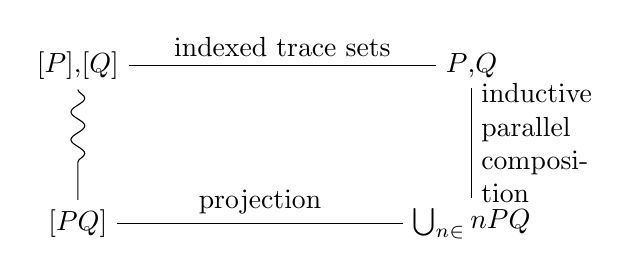
\begin{tikzpicture}
	\node   			(A)	{$\traces[P]$,$\traces[Q]$};
	\node[right of=A, xshift=40mm]	(B)	{$\trI{P}$,$\trI{Q}$};
	\node[below of=B, yshift=-10mm]		(C)	{$\bigcup_{n\in\N}\tracesI{n}{P}{Q}$};
	\node[below of=A, yshift=-10mm]		(D)	{$\traces[\procpar{P}{Q}]$};
	\path	(A)    edge node[anchor=south]  {indexed trace sets}            (B)
		(B)    edge node[anchor=west, text width=15mm]   {inductive parallel composition}    (C)
		(C)    edge node[anchor=south]  {projection}		(D);
	\path	(A)    edge[draw,decorate,decoration={snake, post=lineto, post length=4mm}] 
			    node[anchor=east]   {} (D);
\end{tikzpicture}
\caption{Visualization of the compositionality of the parallel operator (Part I).}
\label{fig_exp_comp_para}
\end{figure}


The behavior of a parallel composition of two processes is their interleaving behavior and the behavior originated from the possible communications between those two processes. For the calculation of the behavior of a parallel composition it is very helpful that we only investigate processes without any restriction operators. Thus, no bound action can exist in any trace. Hence, we neither have to attend to the side condition of the \eparl{} respectively \eparr{} rule for the interleaving behavior nor mind the \eclosel{} respectively \ecloser{} rule of \refFig{fig_ts_early} for the communication case.

Note that for the construction of the additional behavior originated of the communications, we do not have the same problem as described for the case of an input process. This is because in this case, we do have the information to which process the actions belong by calculating the communication behavior.

Following the intuition, we first inductively define the \findex{inductive parallel composition} of a parallel composition by using the indexed trace sets of the components. That is, we memorize from which trace of the one and the other process in the parallel composition the trace of the parallel composed process is constructed and how many of the actions from the traces are used for this construction.

\begin{definition}[Inductive parallel composition]
\label{def_idx_trace_sets}
Let $P,Q\in\procsresf\cap\procsrecf$. Then the function family $\traces_n:\procs_\alpha \rightarrow \pom{(\N^2\times\N^2)\times\tr}$ is defined with
\begin{align*}
	 \tracesI{0}{P}{Q} \define& \set[i_P,i_Q\in\N]{\left(\left(\left(i_P,0\right),\left(i_Q,0\right)\right),\eseq\right)} \\
	 \tracesI{n+1}{P}{Q} \define& \bigl\{\left(\left(\left(i_P,j_P\right),\left(i_Q,j_Q\right)\right),s'\right)\in (\N^2\times\N^2)\times\tr \; \mid \; \\
		& \quad\quad\exists\left(\left(\left(i_P,j_P'\right),\left(i_Q,j_Q'\right)\right),t'\right)\in\tracesI{n}{P}{Q}, \\
		& \quad\quad\quad \left(i_P,s\right)\in\trI{P}, \left(i_Q,t\right)\in\trI{Q}: \\
		& \quad\quad \text{PL}\define\left(j_P=j_P'+1\wedge j_Q=j_Q'\wedge s'=\seqconc{t'}{\seq{s_{j_P}}}\right) \\
		& \quad\wedge \text{PR}\define\left(j_P=j_P'\wedge j_Q=j_Q'+1\wedge s'=\seqconc{t'}{\seq{t_{j_Q}}}\right)  \\
		& \quad\wedge \text{COM}\define\left(j_P=j_P'+1\wedge j_Q=j_Q'+1\wedge s_{j_P}=\conj{t_{j_Q}}\wedge s'=t'\right)\\
		& \quad\wedge \left(\text{PR} \vee \text{PL} \vee \text{COM}\right) \bigr\}
\end{align*}
by induction over $n\in\N$.
\end{definition}

Thus, for a trace $t\in\tr$ of a parallel composition $\procpar{P}{Q}\in\procsresf\cap\procsrecf$, we save the index $i_P$ as well as the index $i_Q$ to memorize from which trace of $P$ respectively $Q$ the trace $t$ is constructed. Additionally, we save with $j_P$ and $j_Q$ the index within the trace of $P$ respectively $Q$, till this index the trace is used for the construction.

Note that the index of the sets does not map the length of the containing traces, since with the conjunctive clause COM every $\tau$ step raises the index, but does not extend the trace. We just can say that for a trace $t\in\tracesI{n}{P}{Q}$ the inequality $\len{t}\leq{}n$ holds. Moreover, the index $n$ counts the inference steps of the operational semantics which had been done to reach the actual tuple of indices and trace.

We now connect this definition to the big-step semantics to have a tool for proving the compositionality of the parallel composition of restriction and recursion free processes.

\begin{lemma}[Inductive parallel composition with big-step semantics]
\label{lem_idx_trace_sets}
$\quad$\newline{}Let $P,Q\in\procsresf\cap\procsrecf$. Then for all $n\in\N\setminus\set{0}$:\newline
\newline
if a tuple $\left(\left(\left(i_P,j_P\right),\left(i_Q,j_Q\right)\right),s'\right)\in\tracesI{n}{P}{Q}$ exists, then there are tuples
\begin{align*}
  \left(\left(\left(i_P,j_P'\right),\left(i_Q,j_Q'\right)\right),t'\right)&\in\tracesI{n-1}{P}{Q}, \\
  \left(i_P,s\right)&\in\trI{P},\\
  \left(i_Q,t\right)&\in\trI{Q}
\end{align*}
such that
\begin{align*}
	&\bigl(j_P=j_P'+1\wedge j_Q=j_Q'\wedge s'=\seqconc{t'}{\seq{s_{j_P}}}\wedge\exists P_1,P_2,Q_1\in\procs: \\
 &\quad\ec{P}\bigstep{\seq{s_1,\ldots,s_{j_P}}}\ec{P_2}\wedge \ec{Q}\bigstep{\seq{t_1,\ldots,t_{j_Q}}}\ec{Q_1}\wedge\ec{\procpar{P}{Q}}\bigstep{t'}\ec{\procpar{P_1}{Q_1}}\transs{s_{j_P}}\ec{\procpar{P_2}{Q_1}}\bigr) \\
	\vee&  \bigl(j_P=j_P'\wedge j_Q=j_Q'+1\wedge s'=\seqconc{t'}{\seq{t_{j_Q}}}\wedge\exists P_1,Q_1,Q_2\in\procs:\\
&\quad \ec{P}\bigstep{\seq{s_1,\ldots,s_{j_P}}}\ec{P_1}\wedge \ec{Q}\bigstep{\seq{t_1,\ldots,t_{j_Q}}}\ec{Q_2}\wedge\ec{\procpar{P}{Q}}\bigstep{t'}\ec{\procpar{P_1}{Q_1}}\transs{t_{j_Q}}\ec{\procpar{P_1}{Q_2}} \bigr) \\
	\vee&  \bigl(j_P=j_P'+1\wedge j_Q=j_Q'+1\wedge s_{j_P}=\conj{t_{j_Q}}\wedge s'=t'\wedge\exists P_1,P_2,Q_1,Q_2\in\procs: \\
&\quad \ec{P}\bigstep{\seq{s_1,\ldots,s_{j_P}}}\ec{P_2}\wedge \ec{Q}\bigstep{\seq{t_1,\ldots,t_{j_Q}}}\ec{Q_2}\wedge \ec{\procpar{P}{Q}}\bigstep{t'}\ec{\procpar{P_1}{Q_1}}\tautrans\ec{\procpar{P_2}{Q_2}}\bigr)
\end{align*}
holds.
\end{lemma}
\begin{prf}
Let $P,Q\in\procsresf\cap\procsrecf$. So we know that neither a restriction operator nor a recursive call occurs in the given processes. Then we prove \refLem{lem_idx_trace_sets} by induction over the index of the inductive parallel composition sets.
\begin{description}
\item[Base case $n=1$:] Let $\left(\left(\left(i_P,j_P\right),\left(i_Q,j_Q\right)\right),s'\right)\in\tracesI{1}{P}{Q}$. From the definition of $\traces_1$, we know there are tuple $\left(\left(\left(i_P,j_P'\right),\left(i_Q,j_Q'\right)\right),t'\right)\in\tracesI{0}{P}{Q}$, $\left(i_P,s\right)\in\trI{P}$ and $\left(i_Q,t\right)\in\trI{Q}$ with
\begin{align*}
	&\left(j_P=j_P'+1\wedge j_Q=j_Q'\wedge s'=\seqconc{t'}{\seq{s_{j_P}}}\right) \\
	\vee&\left(j_P=j_P'\wedge j_Q=j_Q'+1\wedge s'=\seqconc{t'}{\seq{t_{j_Q}}}\right)\\
	\vee&\left(j_P=j_P'+1\wedge j_Q=j_Q'+1\wedge s_{j_P}=\conj{t_{j_Q}}\wedge s'=t'\right).
\end{align*}
From the definition of $\traces_0$, we know that $j_P'=j_Q'=0$ and $t'=\eseq$.
	\begin{description}
		\item[Case $\left(j_P=j_P'+1=1\wedge j_Q=j_Q'=0\wedge s'=\seqconc{t'}{\seq{s_{j_P}}}=\seq{s_1}\right)$:] Since $\left(i_P,s\right)\in\trI{P}$ and the trace sets are prefix closed, we know there are processes $P_1,P_2\in\procs$ such that $\ec{P}\bigstep{}\ec{P_1}\transs{s_1}\ec{P_2}$ holds. Furthermore, with the \eparl{} rule, we know that every $\tau$ transition is also possible in a parallel composition. Moreover, since there is no restriction operator within the processes, and so $\bn{s_1}=\emptyset$, we know that also the $s_1$ transition is possible in the parallel context. Hence, $\ec{\procpar{P}{Q}}\bigstep{t'=\eseq{}}\ec{\procpar{P_1}{Q}}\transs{s_{j_P}=s_1}\ec{\procpar{P_2}{Q}}$ holds and furthermore, we know that $\ec{P}\bigstep{\seq{s_1,\ldots,s_{j_P}}=\seq{s_1}}\ec{P_2}$ and since $\seq{t_1,\ldots,t_0}=\eseq$, $\ec{Q}\bigstep{\seq{t_1,\ldots,t_{j_Q}}=\eseq}\ec{Q}$ holds.
		
		\item[Case $\left(j_P=j_P'=0\wedge j_Q=j_Q'+1=1\wedge s'=\seqconc{t'}{\seq{t_{j_Q}}}=\seq{t_1}\right)$:] Analogously to the prior case, by application of the \eparr{} rule.

		\item[Case $\left(j_P=j_P'+1=1\wedge j_Q=j_Q'+1=1\wedge s_{1}=\conj{t_{1}}\wedge s'=t'=\eseq\right)$:] Like in the other cases we know from $\left(i_P,s\right)\in\trI{P}$ and $\left(i_Q,t\right)\in\trI{Q}$ and that trace sets are prefix closed that there exists processes $P_1,P_2,Q_1,Q_2\in\procs$, with $\ec{P}\bigstep{}\ec{P_1}\transs{s_1}\ec{P_2}$ and $\ec{Q}\bigstep{}\ec{Q_1}\transs{t_1}\ec{Q_2}$. Hence, with the \eparl{} and \eparr{} rule we know $\ec{\procpar{P}{Q}}\bigstep{}\ec{\procpar{P_1}{Q_1}}$ holds and since $s_1=\conj{t_1}$, we know, with the \ecoml{} (respectively \ecomr{}) rule, that $\ec{\procpar{P_1}{Q_1}}\tautrans{}\ec{\procpar{P_2}{Q_2}}$ holds. So all in all we know $\ec{\procpar{P}{Q}}\bigstep{t'=\eseq}\ec{\procpar{P_1}{Q_1}}\tautrans{}\ec{\procpar{P_2}{Q_2}}$ and in addition to that, $\ec{P}\bigstep{\seq{s_1,\ldots,s_{j_P}}=\seq{s_1}}\ec{P_2}$ and $\ec{Q}\bigstep{\seq{t_1,\ldots,t_{j_Q}}=\seq{t_1}}\ec{Q_2}$ holds. 
	\end{description}

\item[Induction hypothesis:] For a given $n\in\N\setminus\set{0}$ \refLem{lem_idx_trace_sets} holds.

\item[Induction step $n\mapsto n+1$:] Let $\left(\left(\left(i_P,j_P\right),\left(i_Q,j_Q\right)\right),s'\right)\in\tracesI{n+1}{P}{Q}$. From the definition of inductive parallel composition set $\traces_{n+1}$ we know there exists tuple $\left(i_P,s\right)\in\trI{P}$, $\left(i_Q,t\right)\in\trI{Q}$, and $\left(\left(\left(i_P,j_P'\right),\left(i_Q,j_Q'\right)\right),t'\right)\in\tracesI{n}{P}{Q}$ such that \begin{equation}
\label{eq_constraint}
	\begin{split}
		&\left(j_P=j_P'+1\wedge j_Q=j_Q'\wedge s'=\seqconc{t'}{\seq{s_{j_P}}}\right) \\
		\vee&\left(j_P=j_P'\wedge j_Q=j_Q'+1\wedge s'=\seqconc{t'}{\seq{t_{j_Q}}}\right)\\
		\vee&\left(j_P=j_P'+1\wedge j_Q=j_Q'+1\wedge s_{j_P}=\conj{t_{j_Q}}\wedge s'=t'\right).
	\end{split}
\end{equation}
holds. Moreover we know from the induction hypothesis that there are tuple $\left(\left(\left(i_P,j_P''\right),\left(i_Q,j_Q''\right)\right),t''\right)\in\tracesI{n-1}{P}{Q}$, $\left(i_P,u\right)\in\trI{P}$ and $\left(i_Q,v\right)\in\trI{Q}$ such that
\begin{align*}
	&\bigl(j_P'=j_P''+1\wedge j_Q'=j_Q''\wedge t'=\seqconc{t''}{\seq{u_{j_P'}}}\wedge\exists{}P_1,P_2,Q_1\in\procs:\\
&\ec{P}\bigstep{\seq{u_1,\ldots,u_{j_P'}}}\ec{P_2}\wedge\ec{Q}\bigstep{\seq{v_1,\ldots,v_{j_Q'}}}\ec{Q_1}\wedge\ec{\procpar{P}{Q}}\bigstep{t''}\ec{\procpar{P_1}{Q_1}}\transs{u_{j_P'}}\ec{\procpar{P_2}{Q_1}}\bigr) \\
	\vee&  \bigl(j_P'=j_P''\wedge j_Q'=j_Q''+1\wedge t'=\seqconc{t''}{\seq{v_{j_Q'}}}\wedge\exists{}P_1,Q_1,Q_2\in\procs: \\
&\ec{P}\bigstep{\seq{u_1,\ldots,u_{j_P'}}}\ec{P_1}\wedge\ec{Q}\bigstep{\seq{v_1,\ldots,v_{j_Q'}}}\ec{Q_2}\wedge\ec{\procpar{P}{Q}}\bigstep{t''}\ec{\procpar{P_1}{Q_1}}\transs{v_{j_Q'}}\ec{\procpar{P_1}{Q_2}}  \bigr) \\
	\vee&  \bigl(j_P'=j_P''+1\wedge j_Q'=j_Q''+1\wedge u_{j_P'}=\conj{v_{j_Q'}}\wedge t'=t''\wedge\exists{}P_1,P_2,Q_1,Q_2\in\procs:\\
&\ec{P}\bigstep{\seq{u_1,\ldots,u_{j_P'}}}\ec{P_2}\wedge \ec{Q}\bigstep{\seq{v_1,\ldots,v_{j_Q'}}}\ec{Q_2}\wedge  \ec{\procpar{P}{Q}}\bigstep{t''}\ec{\procpar{P_1}{Q_1}}\tautrans\ec{\procpar{P_2}{Q_2}}\bigr).
\end{align*}
holds. Hence, we know in every case there are processes $P_2,Q_2\in\procs$ such that $\ec{P}\bigstep{\seq{u_1,\ldots,u_{j_P'}}}\ec{P_2}$, $\ec{Q}\bigstep{\seq{v_1,\ldots,v_{j_Q'}}}\ec{Q_2}$ and $\ec{\procpar{P}{Q}}\bigstep{t'}\ec{\procpar{P_2}{Q_2}}$ holds. Furthermore, since $\left(i_P,s\right)\in\trI{P}$ and $\left(i_P,u\right)\in\trI{P}$ and the indexing of the traces is unique, we know that $s=u$ and also $t=v$ holds. Since Formula \ref{eq_constraint} holds, we again consider three cases:
\begin{description}
		\item[Case $\left(j_P=j_P'+1\wedge j_Q=j_Q'\wedge s'=\seqconc{t'}{\seq{s_{j_P}}}\right)$:] Since $\left(i_P,s\right)\in\trI{P}$ and the trace sets are prefix closed and additionally $j_p=j_P'+1$ we know there exists a process $P_3\in\procs$, such that $\ec{P}\bigstep{\seq{s_1,\ldots,s_{j_p'}}}\ec{P_2}\transs{s_{j_P}}\ec{P_3}$ holds. Again, with the \eparl{} rule and the same arguments as within the base case, we know that the $s_{j_P}$ transition is possible in the parallel context. Hence, $\ec{\procpar{P}{Q}}\bigstep{t'}\ec{\procpar{P_2}{Q_2}}\transs{s_{j_P}}\ec{\procpar{P_3}{Q_2}}$ holds and furthermore, we know that $\ec{P}\bigstep{\seq{s_1,\ldots,s_{j_P}}}\ec{P_3}$ and $\ec{Q}\bigstep{\seq{t_1,\ldots,t_{j_Q}}}\ec{Q_2}$ holds, since $j_Q=j_Q'$.
		
		\item[Case $\left(j_P=j_P'\wedge j_Q=j_Q'+1\wedge s'=\seqconc{t'}{\seq{t_{j_Q}}}\right)$:] This is again proved similarly to the prior case, by application of the \eparr{} rule.

		\item[Case $\left(j_P=j_P'+1\wedge j_Q=j_Q'+1\wedge s_{j_P}=\conj{t_{j_Q}}\wedge s'=t'\right)$:] Like within the other cases, we know from $\left(i_P,s\right)\in\trI{P}$ and $\left(i_Q,t\right)\in\trI{Q}$ and that trace sets are prefix closed that there exists processes $P_3,Q_3\in\procs$, with $\ec{P}\bigstep{\seq{s_1,\ldots,s_{j_P'}}}\ec{P_2}\transs{s_{j_P}}\ec{P_3}$ and $\ec{Q}\bigstep{\seq{t_1,\ldots,t_{j_Q'}}}\ec{Q_2}\transs{t_{j_Q}}\ec{Q_3}$. Since $s_{j_P}=\conj{t_{j_Q}}$ holds, we know with the \ecoml{} (respectively \ecomr{}) rule that $\ec{\procpar{P_2}{Q_2}}\tautrans{}\ec{\procpar{P_3}{Q_3}}$. So again $\ec{\procpar{P}{Q}}\bigstep{t'}\ec{\procpar{P_2}{Q_2}}\tautrans{}\ec{\procpar{P_3}{Q_3}}$ holds.
	\end{description}
\end{description}
So we proved by induction that \refLem{lem_idx_trace_sets} holds for every $n\in\N\setminus\set{0}$.
\end{prf}

Furthermore, all of this behavior is invertible. We know about the traces of a parallel composition that they have to be inferred from the rules of \refFig{fig_ts_early}. Therefore, we can follow every inference step and raise the related counter to receive the inductive parallel composition. Now we know
\[\trI{P}=\set[\exists{}j\in\N:\left(\left(i_P,j\right),\left(i_Q,0\right),s\right)\in\bigcup_{n\in\N}\tracesI{n}{P}{Q}]{\left(i_P,s\right)\in\N\times\tr}\]
and similarly for $\trI{Q}$. Thus, we can gain the traces of $P$ and $Q$ by a projection. This idea is visualized in \refFig{fig_exp_comp_para2}.

% mainfile: ../Refinement.tex
\begin{figure}[h]
\centering
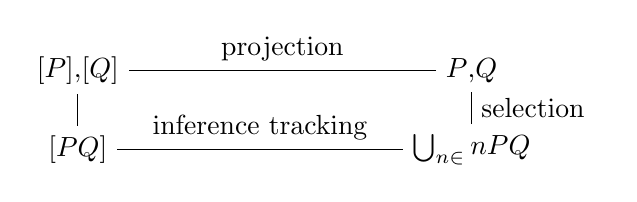
\begin{tikzpicture}
	\node   			(A)	{$\traces[P]$,$\traces[Q]$};
	\node[right of=A, xshift=40mm]	(B)	{$\trI{P}$,$\trI{Q}$};
	\node[below of=B]		(C)	{$\bigcup_{n\in\N}\tracesI{n}{P}{Q}$};
	\node[below of=A]		(D)	{$\traces[\procpar{P}{Q}]$};
	\path	(B)    edge node[anchor=south]  {projection}            (A)
		(C)    edge node[anchor=west, text width=15mm]   {selection}    (B)
		(D)    edge node[anchor=south]  {inference tracking}		(C);
	\path   (D)    edge[draw,decorate,decoration={snake, post=lineto, post length=4mm}] 
			    node[anchor=east]   {} (A);
\end{tikzpicture}
\caption{Visualization of the compositionality of the parallel operator (Part II).}
\label{fig_exp_comp_para2}
\end{figure}


With \refLem{lem_idx_trace_sets} we can show that there is a trace equality such that the traces of the parallel composition of processes without restriction and recursion is equal to the traces within the union of the inductive parallel composition sets.

\begin{lemma}[Compositionality of parallel composition]
\label{lem_compositionality_traces_para}
Given two processes $P,Q\in\procsresf\cap\procsrecf$. Then for the traces of a parallel composition
\[\traces[\procpar{P}{Q}]=\set[\exists\left(\cdot,s\right)\in\bigcup_{n\in\N}\tracesI{n}{P}{Q}]{s\in\tr}\]
holds.
\end{lemma}
\begin{prf}
Let $P,Q\in\procsresf\cap\procsrecf$. For the $\supseteq$-inclusion we know from \refLem{lem_idx_trace_sets} that for all $t\in\set[\exists\left(\cdot,s\right)\in\bigcup_{n\in\N\setminus\set{0}}\tracesI{n}{P}{Q}]{s\in\tr}$ there are $P_2,Q_2\in\procs$ such that $\ec{\procpar{P}{Q}}\bigstep{t}\ec{\procpar{P_2}{Q_2}}$ and so $t\in\traces[\procpar{P}{Q}]$ holds. Since with $t\in\set[\exists\left(\cdot,s\right)\in\tracesI{0}{P}{Q}]{s\in\tr}$ follows $t=\eseq$ and from \refLem{lem_empty_trace} we know that the empty trace is included in every trace set, we know that the fully inclusion holds.

%%%%%%%%%%%%%%%%%%%%%%%%%%%%%%%%%%%%%%%%%%%%%%%%%%%%% OTHER INCLUSION %%%%%%%%%%%%%%%%%%%%%%%%%%%%%%%%%%%%%%%%%%%%%%%%%%%%%%%%%%%%%%%%%%%%%%

For the $\subseteq$-inclusion, we induce over the length of a trace $s\in\traces[\procpar{P}{Q}]$:
\begin{description}
\item[Base case $s=\eseq$:] Since $\tracesI{0}{P}{Q} = \set[i_P,i_Q\in\N]{\left(\left(\left(i_P,0\right),\left(i_Q,0\right)\right),\eseq\right)}$, we know $s\in\set[\exists\left(\cdot,t\right)\in\bigcup_{n\in\N}\tracesI{n}{P}{Q}]{t\in\tr}$.

\item[Base case $s=\seq{\alpha}$ with $\alpha\in\actions\setminus\set{\tau}$:] From the definition of the big-step semantics (\refDef{def_bigstep_semantics}) we know that there are processes $P_1,P_2,Q_1,Q_2\in\procs$ such that $\ec{\procpar{P}{Q}}\bigstep{}\ec{\procpar{P_1}{Q_1}}\transs{\alpha}\ec{\procpar{P_2}{Q_2}}$. Since we have no restriction operator, we know the $\tau$ transitions within $\ec{\procpar{P}{Q}}\bigstep{}\ec{\procpar{P_1}{Q_1}}$ can either be produced from the \ecoml{} (respectively \ecomr{}) rule or from a $\tau$ prefix with the \eparl{} (respectively \eparr{}) rule. So there is a number $m\in\N$ and actions $\alpha_1,\ldots,\alpha_m\in\actions\setminus\set{\tau}$ and $\beta_1,\ldots,\beta_m\in\actions\setminus\set{\tau}$ such that $\ec{P}\bigstep{\seq{\alpha_1,\ldots,\alpha_m}}\ec{P_1}$ and $\ec{Q}\bigstep{\seq{\beta_1,\ldots,\beta_m}}\ec{Q_1}$ holds. Furthermore, there are just the \eparl{} and \eparr{} rule, which can produce the visible action $\alpha$. So we know $\ec{P_1}\transs{\alpha}\ec{P_2}$ or $\ec{Q_1}\transs{\alpha}\ec{Q_2}$ holds. Since both cases can be handled analogously, we just describe the first case. In this case we know $\ec{P}\bigstep{\seq{\alpha_1,\ldots,\alpha_m, \alpha}}\ec{P_2}$ and $Q_1=Q_2$ holds. Hence, there are numbers $i_P,i_Q\in\N$ with $\left(i_P,\seq{\alpha_1,\ldots,\alpha_m,\alpha}\right)\in\trI{P}$ and $\left(i_Q,\seq{\beta_1,\ldots,\beta_m}\right)\in\trI{Q}$. We also know that $\left(\left(\left(i_P,0\right),\left(i_Q,0\right)\right),\eseq\right)\in\tracesI{0}{P}{Q}$ holds so that we can step by step raise the counter for every $\alpha_i$ and $\beta_i$ with $i\in\set{1,\ldots,m}$ by taking in every step the COM conjunctive clause of \refDef{def_idx_trace_sets}. Hence, $\left(\left(\left(i_P,m\right),\left(i_Q,m\right)\right),\eseq\right)\in\tracesI{m}{P}{Q}$ holds. So we see that there is a tuple $\left(\left(\left(i_P,m+1\right),\left(i_Q,m\right)\right),\seq{\alpha}\right)\in\tracesI{m+1}{P}{Q}$, because the PL conjunctive clause of the definition of $\mathcal T_{m+1}$ is fulfilled. So we know $s\in\set[\exists\left(\cdot,t\right)\in\bigcup_{n\in\N}\tracesI{n}{P}{Q}]{t\in\tr}$ holds.

\item[Induction hypothesis:] For a given $n\in\N$, we know that for all $s\in\traces[\procpar{P}{Q}]$ with $\#(s)\leq{}n$ holds that $s\in\set[\exists\left(\cdot,t\right)\in\bigcup_{n\in\N}\tracesI{n}{P}{Q}]{t\in\tr}$.

\item[Induction step $n\mapsto n+1$:] So $\len{s}=n+1$. Again we know from the definition of the big-step semantics that there are processes $P_1,P_2,Q_1,Q_2\in\procs$ such that $\ec{\procpar{P}{Q}}\bigstep{s'}\ec{\procpar{P_1}{Q_1}}\transs{s_{n+1}}\ec{\procpar{P_2}{Q_2}}$ with $s'=\seq{s_1,\ldots,s_n}$ and $s_{n+1}\neq\tau$. Furthermore, since the cases of the empty trace and a trace with just one visible action are already done in the base cases, we consider $\len{s}\geq2$. Hence, we know $s'\neq\eseq$ holds. So there have to be processes $P_1',P_2',Q_1',Q_2'\in\procs$ with $\ec{\procpar{P}{Q}}\bigstep{\seq{s_1,\ldots,s_{n-1}}}\ec{\procpar{P_1'}{Q_1'}}\transs{s_n}\ec{\procpar{P_2'}{Q_2'}}\bigstep{}\ec{\procpar{P_1}{Q_1}}\transs{s_{n+1}}\ec{\procpar{P_2}{Q_2}}$. We now would like to find the suitable indices for $\left(\cdot,s'\right)\in\tracesI{x}{P}{Q}$ so that with this indices really the case $\ec{\procpar{P}{Q}}\bigstep{\seq{s_1,\ldots,s_{n-1}}}\ec{\procpar{P_1'}{Q_1'}}\transs{s_n}\ec{\procpar{P_2'}{Q_2'}}$ is described. So the visible action is the last step of the deduction and $P_2'$ and $Q_2'$ are really reached.

Since $\ec{\procpar{P}{Q}}\bigstep{s'}\ec{\procpar{P_1}{Q_1}}$ holds, we know with the induction hypothesis that $s'\in\set[\exists\left(\cdot,t\right)\in\bigcup_{n\in\N}\tracesI{n}{P}{Q}]{t\in\tr}$. Since $s'\neq\eseq{}$, we know there are $k_P,l_P,k_Q,l_Q,n'\in\N\setminus\set{0}$ such that $\left(\left(\left(k_P,l_P\right),\left(k_Q,l_Q\right)\right),s'\right)\in\tracesI{n'}{P}{Q}$. So, from \refLem{lem_idx_trace_sets}, we know there are tuple $\left(\left(\left(k_P,l_P'\right),\left(k_Q,l_Q'\right)\right),t'\right)\in\tracesI{n'-1}{P}{Q}$, $\left(k_P,r\right)\in\trI{P}$ and $\left(k_Q,t\right)\in\trI{Q}$ such that
\begin{align*}
	&\bigl(l_P=l_P'+1\wedge l_Q=b_Q'\wedge s'=\seqconc{t'}{\seq{r_{l_P}}}\wedge\exists R_1,R_2,S_1\in\procs: \\
 &\quad\ec{P}\bigstep{\seq{r_1,\ldots,r_{l_P}}}\ec{R_2}\wedge \ec{Q}\bigstep{\seq{t_1,\ldots,t_{l_Q}}}\ec{S_1}\wedge\ec{\procpar{P}{Q}}\bigstep{t'}\ec{\procpar{R_1}{S_1}}\transs{r_{l_P}}\ec{\procpar{R_2}{S_1}}\bigr) \\
	\vee&  \bigl(l_P=l_P'\wedge l_Q=l_Q'+1\wedge s'=\seqconc{t'}{\seq{t_{l_Q}}}\wedge\exists R_1,S_1,S_2\in\procs:\\
&\quad \ec{P}\bigstep{\seq{r_1,\ldots,r_{l_P}}}\ec{R_1}\wedge \ec{Q}\bigstep{\seq{t_1,\ldots,t_{l_Q}}}\ec{S_2}\wedge\ec{\procpar{P}{Q}}\bigstep{t'}\ec{\procpar{R_1}{S_1}}\transs{t_{l_Q}}\ec{\procpar{R_1}{S_2}} \bigr) \\
	\vee&  \bigl(l_P=l_P'+1\wedge l_Q=l_Q'+1\wedge r_{l_P}=\conj{t_{l_Q}}\wedge s'=t'\wedge\exists R_1,R_2,S_1,S_2\in\procs: \\
&\quad \ec{P}\bigstep{\seq{r_1,\ldots,r_{l_P}}}\ec{R_2}\wedge \ec{Q}\bigstep{\seq{t_1,\ldots,t_{l_Q}}}\ec{S_2}\wedge \ec{\procpar{P}{Q}}\bigstep{t'}\ec{\procpar{R_1}{S_1}}\tautrans\ec{\procpar{R_2}{S_2}}\bigr)
\end{align*}
holds. Hence, we know there are processes $R_2,S_2\in\procs$ with $\ec{\procpar{P}{Q}}\bigstep{s'}\ec{\procpar{R_2}{S_2}}$, but we do not know if these are the right indices such that $R_2=P_2'$, $S_2=Q_2'$ holds and $s_n$ is really the last deduction step. This is because arbitrary many $\tau$ steps could be performed after the visible action $s_n$ with the COM conjunctive clause of \refDef{def_idx_trace_sets} and nevertheless $s'\in\set[\exists\left(\cdot,t\right)\in\bigcup_{n\in\N}\tracesI{n}{P}{Q}]{t\in\tr}$ would hold. But we can revert every of the excessive $\tau$ steps, so we know there exists $m,j_P',j_P'',j_Q',j_Q''\in\N$ with $m\leq{}n'$,$j_P''\leq{}l_P'$ and $j_Q''\leq{}l_Q'$ such that $\left(\left(\left(k_P,j_P'\right),\left(k_Q,j_Q'\right)\right),s'\right)\in\tracesI{m}{P}{Q}$, $\left(\left(\left(k_P,j_P''\right),\left(k_Q,j_Q''\right)\right),t'\right)\in\tracesI{m-1}{P}{Q}$, $\left(k_P,r\right)\in\trI{P}$ and $\left(k_Q,t\right)\in\trI{Q}$ exists such that
\begin{align*}
	&\bigl(j_P'=j_P''+1\wedge j_Q'=j_Q''\wedge r_{j_P'}=s_n \wedge s'=\seqconc{t'}{\seq{s_n}} \\
&\quad\wedge\ec{P}\bigstep{\seq{r_1,\ldots,r_{j_P'}}}\ec{P_2'}\wedge \ec{Q}\bigstep{\seq{t_1,\ldots,t_{j_Q'}}}\ec{Q_1'}\wedge\ec{\procpar{P}{Q}}\bigstep{t'}\ec{\procpar{P_1'}{Q_1'}}\transs{s_n}\ec{\procpar{P_2'}{Q_1'}}\bigr)\\
\vee&  \bigl(j_P'=j_P''\wedge j_Q'=j_Q''+1\wedge t_{j_Q'}=s_n \wedge s'=\seqconc{t'}{\seq{s_n}} \\
&\quad \wedge \ec{P}\bigstep{\seq{r_1,\ldots,r_{j_P'}}}\ec{P_1'}\wedge \ec{Q}\bigstep{\seq{t_1,\ldots,t_{j_Q'}}}\ec{Q_2'}\wedge\ec{\procpar{P}{Q}}\bigstep{t'}\ec{\procpar{P_1'}{Q_1'}}\transs{s_n}\ec{\procpar{P_1'}{Q_2'}} \bigr)
\end{align*}
holds. The conjunctive clause which handles the communication case is not satisfiable since the last step has to be a visible action and is due to that omitted.

Since $t'=\seq{s_1,\ldots,s_{n-1}}$, we found the suitable indices such that 
\[\ec{\procpar{P}{Q}}\bigstep{\seq{s_1,\ldots,s_{n-1}}}\ec{\procpar{P_1'}{Q_1'}}\transs{s_n}\ec{\procpar{P_2'}{Q_2'}}\]
holds. We now have to raise the indices for the $\tau$ steps within $\ec{\procpar{P_2'}{Q_2'}}\bigstep{}\ec{\procpar{P_1}{Q_1}}$ and the visible action $\ec{\procpar{P_1}{Q_1}}\transs{s_{n+1}}\ec{\procpar{P_2}{Q_2}}$. Again we know that the visible action $s_{n+1}$ must be produced from the \eparl{} (respectively \eparr{}) rule and since both cases are similar, we concentrate on the \eparl{} case.

To find the suitable indices such that $\ec{\procpar{P}{Q}}\bigstep{s'}\ec{\procpar{P_2'}{Q_2'}}\bigstep{}\ec{\procpar{P_1}{Q_1}}\transs{s_{n+1}}\ec{\procpar{P_2}{Q_2}}$ holds, we can -- as in the second base case -- raise the indices for every $\tau$ step within $\ec{\procpar{P_2'}{Q_2'}}\bigstep{}\ec{\procpar{P_1}{Q_1}}$ with the COM conjunctive clause. But in this case, we do not know, how $r$ and $t$ look like. If they are long enough so that every action which is needed in the premise of the \ecoml{} (respectively \ecomr{}) rule to deduct the $\tau$ steps within $\ec{\procpar{P_2'}{Q_2'}}\bigstep{}\ec{\procpar{P_1}{Q_1}}$ and as well the action $s_{n+1}$ is contained, then we can just raise the counter. Otherwise, if $r$ and $t$ do not contain every needed action, we know $\ec{\procpar{P}{Q}}\bigstep{\seq{s_1,\ldots,s_{n-1}}}\ec{\procpar{P_1'}{Q_1'}}\transs{s_n}\ec{\procpar{P_2'}{Q_2'}}\bigstep{}\ec{\procpar{P_1}{Q_1}}\transs{s_{n+1}}\ec{\procpar{P_2}{Q_2}}$ holds and that those steps can just be performed by applying the \eparl{} (respectively \eparr{}) or \ecoml{} (respectively \ecomr) rules. Hence, we know, there have to be traces $u,v\in\tr$ with $\ec{P}\bigstep{r}\ec{P_2'}\bigstep{\seqconc{u}{\seq{s_{n+1}}}}\ec{P_2}$ and $\ec{Q}\bigstep{t}\ec{Q_2'}\bigstep{v}\ec{Q_2}$, since we consider the \eparl{} case. Hence, we know that nothing changes, if we use the tuple $\left(i_P,u'\right)\in\trI{P}$ with $u'\define\seqconc{\seqconc{r}{u}}{s_{n+1}}$ instead of $\left(k_P,r\right)\in\trI{P}$ and $\left(i_Q,v'\right)\in\trI{Q}$ with $v'\define\seqconc{t}{v}$ instead of $\left(k_Q,t\right)\in\trI{Q}$. With this we can, as in the base case, increase $j_P'$ and $j_Q'$ by one for every $\tau$ deduction within $\ec{\procpar{P_2'}{Q_2'}}\bigstep{}\ec{\procpar{P_1}{Q_1}}$. So we found the suitable numbers $m',i_P,j_P,i_Q,j_Q\in\N$ such that $\left(\left(\left(i_P,j_P\right),\left(i_Q,j_Q\right)\right),s'\right)\in\tracesI{m'}{P}{Q}$, $\left(i_P,u'\right)\in\trI{P}$ and $\left(i_Q,v'\right)\in\trI{Q}$, with $m'\geq{}m$, $j_P\geq{}j_P'$ and $j_Q\geq{}j_Q'$ holds for $\ec{\procpar{P}{Q}}\bigstep{\seq{s_1,\ldots,s_{n-1}}}\ec{\procpar{P_1'}{Q_1'}}\transs{s_n}\ec{\procpar{P_2'}{Q_2'}}\bigstep{}\ec{\procpar{P_1}{Q_1}}$. Hence, we know that $\left(\left(\left(i_P,j_P+1\right),\left(i_Q,j_Q\right)\right),s\right)\in\tracesI{m'+1}{P}{Q}$ holds, since the PL conjunctive clause holds, because of considering the \eparl{} case. So $s\in\set[\exists\left(\cdot,t\right)\in\bigcup_{n\in\N}\tracesI{n}{P}{Q}]{t\in\tr}$ holds.
\end{description}
So we proved that the parallel composition is compositional for processes without restriction and recursion.
\end{prf}

The next section dealts with the last unconsidered operator of recursion-free \picalc{} processes.


% mainfile: ../../Refinement.tex
\subsubsection{Restriction}
\label{sec_comp_res}
To show an idea for the compositionality of the trace semantics for the restriction operator, we firstly define a function called \findex{restriction set} for two names and a set of traces. The idea of this approach is to take the traces of $P$ for a process $\procres{a}{P}$ and replace the name $a$ by every fresh name $a'\nin\fn{P}$. This does not cause any trouble because of \refLem{lem_subst_trace_partII} respectively \refLem{lem_subst_bigstep_partIII} and \refLem{lem_subst_bigstep_partIV}. We have to consider every $a'\nin\fn{P}$ since we know that $\procres[()]{a'}{P\subs{a'}{a}}\in\ec{\procres{a}{P}}$ holds for all of such $a'$. Then, we can change the first occurrence of an output action $\outa{x}{a'}$ to $\bouta{x}{a'}$ if existent. This yields from the \eopen{} rule of \refFig{fig_ts_early} and from \refConv{conv_uni_bn_traces}. After that work is done, we can filter out the desired traces. That is, we know that after an application of the \eopen{} rule the restriction operator is omitted, thus every possible behavior is allowed. Otherwise, the name $a'$ is not allowed to occur as subject of an action. Hence, we only collect those traces, where something is send over the channel $a'$ if $a'$ has firstly been an object of a bound output action. The proof of the equality of the union of this restriction sets to the trace set of the restricted process, is not completely finish. So we only give ideas and limitations for this case.  %This idea leads to the definition of the \findex{restriction set} for two names and a set of traces.

\begin{old}[Old trace association which does not hold] %%%%%%%%%%%%%%%%%%%%%%%%%%%%%%%%%%%%%%%%%%%%%%%%%%%%%%%%%%%%%%%%%%%%% OLD
\todo[inline]{Beschreibe warum am Beispiel Problem wenn a nicht der restricted name zu dem Trace ist. Deswegen Def. dann beweisen, dass es so einen namen a immer gibt. Der ist nur nicht eindeutig}
\begin{definition}[Trace-Process association]\index{trace-process association}
\label{def_trace_belonging}\todo{evtl. no negation?}
Given a name $a\in\names$ and a process $P\in\procs$. We say a trace $t\in\traces[\procres{a}{P}]$ \findex[trace!belongs to process]{belongs} to the process $\procres{a}{P}$ or the process $\procres{a}{P}$ is \index{association}\findex[trace!associated to process]{associated} to the the trace $t\in\traces[\procres{a}{P}]$ if $\nexists{}x\in\names\setminus\bn{\procres{a}{P}}: t\in\traces[\procres{x}{P\subs{x}{a}}] \wedge x\in\n{t}$ holds.
\end{definition}
That is, $\procres{a}{P}$ is the process out of the equivalence class, which is really used to create the trace $t$ since we cannot find another name such that the name occurs bound in $t$ and we can replace $a$ by it \todo{bla write s.th. meaningful} 
\todo[inline]{restriction to bound names harmful since other bsp zettel}
\end{old} %%%%%%%%%%%%%%%%%%%%%%%%%%%%%%%%%%%%%%%%%%%%%%%%%%%%%%%%%%%%%%%%%%%%% OLD

\begin{definition}[Restriction set]
\label{def_res_set}
For $a,a'\in\names$ and $P\in\procs$ we define $\texttt{res}:\names\times\names\times\pom{\tr}\rightarrow\pom{\tr}$ with
\begin{align*}
	\res{a}{a'}{P}\define&\bigl\{s\in\bind{a'}{\left(\traces[P]\transp{a'}{a}\right)} \;\mid \\
				& \quad \forall{}i\in\N: a'\in\sub{s_i} \Rightarrow \exists{}j\in\N: a'\in\bn{s_j}\wedge{}j<i \bigr\}
\end{align*}
as the \findex{restriction set} of $a$, $a'$, and $\traces[P]$.
\end{definition}
%a function which interchanges $a$ and $a'$ and restricts the name $a'$ to the trace set $\traces[P]$.

%\begin{old}[Not finished proof] %%%%%%%%%%%%%%%%%%%%%%%%%%%%%%%%%%%%%%%%%%%%% NOT FINISHED PROOF %%%%%%%%%%%%%%%%%%%%%%%%%%%%%
%\todo[inline]{ACHTUNG: dieses Lemma konnte ich so nicht zeigen}
%\begin{lemma}[From restriction to restriction set]
%\label{lem_from_res_to_resset}
%Given $a\in\names$, $P,Q\in\procs$ and $t\in\tr$, then
%\begin{align*}
%  \ec{\procres{a}{P}}\bigstep{t}\ec{Q} \text{ implies it exists } a'\in\names\setminus\fn{\procres{a}{P}},Q'\in\procs,s\in\tr
%\end{align*}
%with
%\[t\in\res{a}{a'}{P},\ec{P}\bigstep{s}\ec{Q'}, t=\bind{a'}{s\transp{a'}{a}}\] and 
%\begin{itemize}
%\item[(I)] $\ec{Q}=\ec{\procres[()]{a'}{Q'\transp{a'}{a}}}$ with $a'\nin\n{t}$ or
%\item[(II)] $\ec{Q}=\ec{Q'\transp{a'}{a}}$ with $a'\in\bn{t}$
%\end{itemize}
%holds.
%\end{lemma}
%\begin{prf}
%Let $a\in\names$, $P,Q\in\procs$ and $t\in\traces$ with $\ec{\procres{a}{P}}\bigstep{t}\ec{Q}$. Then we prove \refLem{lem_from_res_to_resset} by induction over the length $n\in\N$ of trace $t$. 
%\begin{description}
%\item[Base case $n=0$:] Hence, $t=\eseq{}$ and so $\ec{\procres{a}{P}}\bigstep{}\ec{Q}$.\todo{ref Lemma, or prove it with more hand-waving here.} This yields $\ec{P}\bigstep{}\ec{Q_1}$ with $\ec{Q}=\ec{\procres{a}{Q_1}}$. We chose $s\define{}\eseq{}$ and $Q'\define{Q_1}$. Hence, $t=\bind{a'}{s\transp{a}{a'}}$ 
%and $\ec{Q}=\ec{\procres{a}{Q'}}=\ec{\procres{a'}{Q'\transp{a'}{a}}}$ with $a'\nin\n{t}$ for all $a'\nin\fn{\procres{a}{P}}$. Thus, $t\in\res{a}{a'}{P}$.

%\item[Induction hypothesis:] For a number $n\in\N$, processes $P,Q\in\procs$, a name $a\in\names$ and a trace $t\in\tr$ with $\len{t}=n$ we know $\ec{\procres{a}{P}}\bigstep{t}\ec{Q}$ implies the existence of $a'\in\names\setminus\fn{\procres{a}{P}},Q'\in\procs,s\in\tr$ with $t\in\res{a}{a'}{P},\ec{P}\bigstep{s}\ec{Q'}, t=\bind{a'}{s\transp{a'}{a}}$ and $\ec{Q}=\ec{\procres[()]{a'}{Q'\transp{a'}{a}}}$ with $a'\nin\n{t}$ or $\ec{Q}=\ec{Q'\transp{a'}{a}}$ with $a'\in\bn{t}$.

%\item[Induction step $n\mapsto n+1$:] Thus, it exists a trace $t'\in\tr$ and a visible action $\alpha\in\actions\setminus\set{\tau}$ with $t=\seqconc{t'}{\seq{\alpha}}$. Hence, there is a process $Q_1\in\procs$ with $\ec{\procres{a}{P}}\bigstep{t'}\ec{Q_1}\bigstep{\seq{\alpha}}\ec{Q}$. The induction hypothesis yields that there is a name $a'\in\names\setminus\fn{\procres{a}{P}}$, a process $Q_1'\in\procs$ and a trace $s'\in\tr$ with $t'\in\res{a}{a'}{P},\ec{P}\bigstep{s'}\ec{Q_1'}, t'=\bind{a'}{s'\transp{a'}{a}}$ and $(I): \ec{Q_1}=\ec{\procres[()]{a'}{Q_1'\transp{a'}{a}}}$ with $a'\nin\n{t'}$ or $(II): \ec{Q_1}=\ec{Q_1'\transp{a'}{a}}$ with $a'\in\bn{t'}$. 
%\begin{description}

%	\item[Case $(I)$:] Since $\ec{Q_1}=\ec{\procres[()]{a'}{Q_1'\transp{a'}{a}}}$ and $\ec{Q_1}\bigstep{\seq{\alpha}}\ec{Q}$ we know there are processes $Q_2, Q_3\in\procs$ with $\ec{\procres[()]{a'}{Q_1'\transp{a'}{a}}}\bigstep{}\ec{Q_2}\transs{\alpha}\ec{Q_3}\bigstep{}\ec{Q}$. As in the base case we do not have to investigate the $\tau$ steps separately, since they preserve the restriction operator and all the other properties. %Furthermore, since there are just two rules in \refFig{fig_ts_early} which produce a transition from a restricted process (the \eres{} and the \eopen{} rule), we know there is either an $x=a'$ such that $\alpha=\bout{x}{a'}$ and or .\todo{Hier fiel mir ein Fehler auf.}
%Thus, there is a process $Q_2'\in\procs$ such that $\ec{\procres[()]{a'}{Q_1'\transp{a'}{a}}}\bigstep{}\ec{\procres[()]{a'}{Q_2'\transp{a'}{a}}}$ and $\ec{Q_1'\transp{a'}{a}}\bigstep{}\ec{Q_2'\transp{a'}{a}}$ with the \eres{} rule of \refFig{fig_ts_early}. With \refLem{lem_subst_bigstep_partIII} we know there is a process $Q_2''\in\procs$ with $\ec{Q_1'}\bigstep{}\ec{Q_2''}$ and $\ec{Q''\transp{a'}{a}}=\ec{Q_2'}$.

%if $a'\nin\n{\alpha}$, then

%if $a'\in\obj{\alpha}$ and it exists $x\in\names$ with $x\neq{}a'$ and $\alpha=\bouta{x}{a'}$, then

%if $a'\in\obj{\alpha}$ and it exists $x\in\names$ with $x\neq{}a'$ and $\alpha=\outa{x}{a'}$, then choose another name for $a'$. \todo{assumption}

%if $a'\in\sub{\alpha}$, then choose another name for $a'$. \todo{assumption}

%	\item[Case $(II)$:] Since $\ec{Q_1}\bigstep{\seq{\alpha}}\ec{Q}$ and $\ec{Q_1}=\ec{Q_1'\transp{a'}{a}}$ we know with \refLem{lem_subst_bigstep_partIV} that there is an action $\alpha'\in\actions$ and a process $Q'\in\procs$ such that $\ec{Q_1'}\bigstep{\seq{\alpha'}}\ec{Q'}$ with $\ec{Q}=\ec{Q'\transp{a'}{a}}$ and $\alpha=\transp{a'}{a}(\alpha')$. Since $\ec{P}\bigstep{s'}\ec{Q_1'}$ we know there is a trace $s\in\tr$ with $\ec{P}\bigstep{s}\ec{Q'}$ and $s=\seqconc{s'}{\seq{\alpha'}}$. Since $a'\in\bn{t'}$ we know $t=\seqconc{t'}{\seq{\alpha}}=\bind{a'}{\seqconc{s'\transp{a'}{a}}{\seq{\alpha}}}=\bind{a'}{(\seqconc{s'}{\seq{\alpha'}})\transp{a'}{a}}=\bind{a'}{s\transp{a'}{a}}$ and $a'\in\bn{t}$. Since $t'\in\res{a}{a'}{P}$ and $a'\in\bn{t'}$ we know $t\in\res{a}{a'}{P}$ holds.
%\end{description}
%\end{description}
%\end{prf}

%\begin{lemma}[Compositionality of restriction (Part I)]
%\label{lem_compositionality_traces_res_I}
%	Given $P\in\procsrecf$ and $a\in\names$, then
%	\[\traces[\procres{a}{P}]\subseteq\bigcup_{a'\in\names\setminus\fn{\procres{a}{P}}}\res{a}{a'}{P}\]
%	holds.
%	%%%%%%%%%%%%%%%%%%%%%%%%%%%%%%%%%%%%%%%%%%%% THIRD VERSION %%%%%%%%%%%%%%%%%%%%%%%%%%%%%%%%%%%%%%%%%%%%%%%%%%%%%%%%%%%%%%%%%%%%%%%%%%%%%%%%
%%	\begin{old}{third version}			
%%	Let $P\in\procsrecf$ and $a\in\names$, then define $T_B\define\bind{a}{\traces[P]}$ and with that define 
%%	\begin{align*}
%%		T_P\define{}T_B\setminus\bigl(&\left\{s\in{}T_B \; \mid \; \exists{}i,j\in\N:a\in\sub{s_i}\wedge{}a\in\obj{s_j}\wedge{}i\leq{}j\right\} \\
%%				&\cup \set[\exists{}i\in\N\;\nexists{}j\in\N:a\in\sub{s_i}\wedge{}a\in{}\obj{s_j}]{s\in{}T_B}\bigr).
%%	\end{align*}
%%	 Then the compositionality of the restriction operator
%%				\[\traces[\procres{a}{P}] = \bigcup_{a'\in\names}\left(\bnsubst{a'}{a}{T_P}\right)\]			
%%	holds.
%%	\end{old}
%%	%%%%%%%%%%%%%%%%%%%%%%%%%%%%%%%%%%%%%%%%%%%% END THIRD VERSION %%%%%%%%%%%%%%%%%%%%%%%%%%%%%%%%%%%%%%%%%%%%%%%%%%%%%%%%%%%%%%%%%%%%%%%%%%%%%
%%	%%%%%%%%%%%%%%%%%%%%%%%%%%%%%%%%%%%%%%%%%%%% THIRD VERSION %%%%%%%%%%%%%%%%%%%%%%%%%%%%%%%%%%%%%%%%%%%%%%%%%%%%%%%%%%%%%%%%%%%%%%%%%%%%%%%%
%%	\begin{old}{third version}			
%%		Let $T_B\define\bind{a}{\traces[P]}$ and with that \newline$T_P\define{}T_B\setminus\bigl(\left\{s\in{}T_B \; \mid \; \exists{}i,j\in\N:a\in\sub{s_i}\wedge{}a\in\obj{s_j}\wedge{}i\leq{}j\right\}$\newline{} $\cup \set[\exists{}i\in\N\nexists{}j\in\N:a\in\sub{s_i}\wedge{}a\in{}\obj{s_j}]{s\in{}T_B}\bigr)$, then
%%%\set[\exists{}i,j\in\N:a\in\sub{s_i}\wedge{}a\in\obj{s_j}\wedge{}i\leq{}j]{s\in{}T_B}
%%			\[\traces[\procres{a}{P}] = \bigcup_{a'\in\names}\left(T_P\subs{a'}{a}\right)\]			
%%	\end{old}
%%	%%%%%%%%%%%%%%%%%%%%%%%%%%%%%%%%%%%%%%%%%%%% END THIRD VERSION %%%%%%%%%%%%%%%%%%%%%%%%%%%%%%%%%%%%%%%%%%%%%%%%%%%%%%%%%%%%%%%%%%%%%%%%%%%%%
%%	%%%%%%%%%%%%%%%%%%%%%%%%%%%%%%%%%%%%%%%%%%%%% SECOND VERSION %%%%%%%%%%%%%%%%%%%%%%%%%%%%%%%%%%%%%%%%%%%%%%%%%%%%%%%%%%%%%%%%%%%%%%%%%%%%%%
%%	\begin{old}{second version}		
%%		Let $T_P\define\traces[P]\setminus\bigl(\set[a\in_c s]{s\in\traces[P]}\cup\set[\out{b}{a}\in s,b\in\names]{s\in\traces[P]}\bigr)\cup \set[{s\in\traces[P]}]{s\subs{\left(a\right)}{\langle{}a\rangle}}$, then
%%					\[\traces[\procres{a}{P}] = \bigcup_{a'\in\names}\left(T_P\subs{a'}{a}\right)\]
%%	\end{old}
%%	%%%%%%%%%%%%%%%%%%%%%%%%%%%%%%%%%%%%%%%%%%%%%% END SECOND VERSION %%%%%%%%%%%%%%%%%%%%%%%%%%%%%%%%%%%%%%%%%%%%%%%%%%%%%%%%%%%%%%%%%%%%%%%%%%%%%%
%%	%%%%%%%%%%%%%%%%%%%%%%%%%%%%%%%%%%%%%%%%%%%%% FIRST VERSION %%%%%%%%%%%%%%%%%%%%%%%%%%%%%%%%%%%%%%%%%%%%%%%%%%%%%%%%%%%%%%%%%%%%%%%%%%%%%%
%%	\begin{old}{first version}		
%%		\begin{align*}
%%			\traces[\procres{a}{P}] \define \bigcup_{a'\in\names}\bigl(\traces[P]\subs{a'}{a}&\setminus\bigl(\set[a'\in_c s]{s\in\traces[P]\subs{a'}{a}} \\
%%							& \quad\quad\cup \set[\out{b}{a'}\in s,b\in\names]{s\in\traces[P]\subs{a'}{a}}\bigr) \\
%%							&\cup \set[{s\in\traces[P]\subs{a'}{a}}]{s\subs{\left(a'\right)}{\langle{}a'\rangle}}\bigr).
%%		\end{align*}
%%	\end{old}
%	%%%%%%%%%%%%%%%%%%%%%%%%%%%%%%%%%%%%%%%%%%%%%% END FIRST VERSION %%%%%%%%%%%%%%%%%%%%%%%%%%%%%%%%%%%%%%%%%%%%%%%%%%%%%%%%%%%%%%%%%%%%%%%%%%%%%%
%\end{lemma}
%\end{old} %%%%%%%%%%%%%%%%%%%%%%%%%%%%%%%%%%%%%%%%%%%%%%%%%%%%%%%% NOT FINISHED PROOF %%%%%%%%%%%%%%%%%%%%%%%%%%%%%%%%%%%%%%

To investigate the equality of a union of restriction sets to the traces of a corresponding restricted process, we list a lemma which reduces one inclusion of this problem to the big-step semantics.

\begin{lemma}[From restriction set to restriction]
\label{lem_from_resset_to_res}
Given $P\in\procsrecf$ and $a\in\names$. For a name $a'\in\names\setminus\fn{\procres{a}{P}}$ we know

\begin{align*}
t\in\res{a}{a'}{P}, \ec{P}\bigstep{s}\ec{Q} \text{ with } t=\bind{a'}{s\transp{a'}{a}} \text{ and }\\
 a'\nin\bn{t}\Rightarrow\nexists{} i\in\N\colon{}a'\in\obj{t_i}\wedge{}t_i\in\inA
\end{align*}
implies
\begin{itemize}
  \item[(I)] $\ec{\procres[()]{a'}{P\transp{a'}{a}}}\bigstep{t}\ec{\procres[()]{a'}{Q\transp{a'}{a}}}$ with $a'\nin\bn{t}$  or
  \item[(II)] $\ec{\procres[()]{a'}{P\transp{a'}{a}}}\bigstep{t}\ec{Q\transp{a'}{a}}$ with $a'\in\bn{t}$
\end{itemize}
holds.
\end{lemma}
\begin{prf}
Let $P\in\procsrecf$, $a\in\names$, $a'\in\names\setminus\fn{\procres{a}{P}}$, $t\in\res{a}{a'}{P}$ and $\ec{P}\bigstep{s}\ec{Q}$ with $t=\bind{a'}{s\transp{a'}{a}}$ and $a'\nin\bn{t}\Rightarrow\nexists{} i\in\names\colon{}a'\in\obj{t_i}\wedge{}t_i\in\inA$. We proceed by induction over the length $n\in\N$ of trace $s$.
\begin{description}
\item[Base case $n=0$:] Hence, $s=\eseq{}$ and so $t=\bind{a'}{\eseq{}\transp{a'}{a}}=\bind{a'}{\eseq}=\eseq{}$. Since $\ec{P}\bigstep{\eseq{}}\ec{Q}$ holds, we know with \refLem{lem_subst_bigstep_partI} that $\ec{P\transp{a'}{a}}\bigstep{\eseq{}}\ec{Q\transp{a'}{a}}$. With multiple application of the \eres{} rule of \refFig{fig_ts_early}, we know $\ec{\procres[()]{a'}{P\transp{a'}{a}}}\bigstep{\eseq{}}\ec{\procres[()]{a'}{Q\transp{a'}{a}}}$ with $a'\nin\n{t}$.

\item[Induction hypothesis:] For an arbitrary number $n\in\N$, we know for all processes $P\in\procs$ and names $a\in\names$ that for a name $a'\in\names\setminus\fn{\procres{a}{P}}$ that if a trace $t\in\res{a}{a'}{P}$ with $t=\bind{a'}{s\transp{a'}{a}}$ such that $a'\nin\bn{t}\Rightarrow\nexists{} i\in\names\colon{}a'\in\obj{t_i}\wedge{}t_i\in\inA$ holds and $\ec{P}\bigstep{s}\ec{Q}$ and $\len{s}\leq{}n$ exists, then $\ec{\procres[()]{a'}{P\transp{a'}{a}}}\bigstep{t}\ec{\procres[()]{a'}{Q\transp{a'}{a}}}$ with $a'\nin\bn{t}$ or $\ec{\procres[()]{a'}{P\transp{a'}{a}}}\bigstep{t}\ec{Q\transp{a'}{a}}$ with $a'\in\bn{t}$ holds.

\item[Induction step $n\mapsto n+1$:] Thus, there is a trace $s'\in\tr$ and a visible action $\alpha'\in\actions\setminus\set{\tau}$ with $s=\seqconc{s'}{\seq{\alpha'}}$. Thus, $t=\bind{a'}{(\seqconc{s'}{\seq{\alpha'}})\transp{a'}{a}}=\bind{a'}{\seqconc{s'\transp{a'}{a}}{\seq{\alpha'}\transp{a'}{a}}}$. Since $\ec{P}\bigstep{s}\ec{Q}$ we know there exists processes $Q_1,Q_2\in\procs$ with $\ec{P}\bigstep{s'}\ec{Q_1}\transs{\alpha'}\ec{Q_2}\bigstep{}\ec{Q}$. With \refConv{conv_uni_bn_traces} we know $a,a'\nin\bn{s'}\cup\bn{\alpha'}$. Let $t'\define\bind{a'}{s'\transp{a'}{a}}$ and $\alpha\define\transp{a'}{a}(\alpha')$. Since $t\in\res{a}{a'}{P}$ and $t'$ is a prefix of $t$ we know $t'\in\res{a}{a'}{P}$ and so the induction hypothesis yields that (I) $\ec{\procres[()]{a'}{P\transp{a'}{a}}}\bigstep{t'}\ec{\procres[()]{a'}{Q_1\transp{a'}{a}}}$ with $a'\nin\bn{t'}$ or (II) $\ec{\procres[()]{a'}{P\transp{a'}{a}}}\bigstep{t'}\ec{Q_1\transp{a'}{a}}$ with $a'\in\bn{t'}$ holds.

\begin{description}
\item[Case $a'\in\bn{t'}$:] Thus, $\ec{\procres[()]{a'}{P\transp{a'}{a}}}\bigstep{t'}\ec{Q_1\transp{a'}{a}}$. Since the $\texttt{bind}$ function just binds the first occurrence of the given name in a trace and leaves the rest of the trace unaltered, $t=\seqconc{t'}{\seq{\alpha}}$ with $\seq{\alpha}\define\seq{\alpha'}\transp{a'}{a}$ and $a'\nin\bn{\alpha}$ holds. Since $\ec{Q_1}\bigstep{\seq{\alpha'}}\ec{Q}$ holds, we know with \refLem{lem_subst_bigstep_partII} that $\ec{Q_1\transp{a'}{a}}\bigstep{\seq{\alpha'}\transp{a'}{a}}\ec{Q\transp{a'}{a}}$ holds and so $\ec{\procres[()]{a'}{P\transp{a'}{a}}}\bigstep{t}\ec{Q\transp{a'}{a}}$. Since, we have seen $a'\in\bn{t'}$ and $a'\nin\bn{\alpha}$, we know $a'\in\bn{t}$.

\item[Case $a'\nin\bn{t'}$:] Hence, $\ec{\procres[()]{a'}{P\transp{a'}{a}}}\bigstep{t'}\ec{\procres[()]{a'}{Q_1\transp{a'}{a}}}$. Furthermore, $t'=s'\transp{a'}{a}$, since $a'\nin\bn{t'}$. Since $\ec{Q_1}\transs{\alpha'}\ec{Q_2}$ we know with \refLem{lem_subst_trans_partI} that $\ec{Q_1\transp{a'}{a}}\transs{\alpha}\ec{Q_2\transp{a'}{a}}$ holds and analogously \refLem{lem_subst_bigstep_partI} yields $\ec{Q_2\transp{a'}{a}}\bigstep{}\ec{Q\transp{a'}{a}}$.

If $a'\nin\n{\alpha}$ the \eres{} rule of \refFig{fig_ts_early} yields $\ec{\procres[()]{a'}{Q_1\transp{a'}{a}}}\transs{\alpha}\ec{\procres[()]{a'}{Q_2\transp{a'}{a}}}$. Similarly, we know with multiple application of the \eres{} rule that $\ec{\procres[()]{a'}{Q_2\transp{a'}{a}}}\bigstep{}\ec{\procres[()]{a'}{Q\transp{a'}{a}}}$ and since $a'\nin\n{\alpha}$ we know $\bind{a'}{\alpha}=\alpha$ and so $\ec{\procres[()]{a'}{P\transp{a'}{a}}}\bigstep{t}\ec{\procres[()]{a'}{Q\transp{a'}{a}}}$ with $a'\nin\bn{t}$.

If $a'\in\n{\alpha}$, we know that $a'\nin\sub{\alpha}$, because otherwise $a'$ must have been bound in $t'$, since $a'\nin\n{t'}$, $t=\seqconc{t'}{\bind{a'}{\seq{\alpha}}}$ and $t\in\res{a}{a'}{P}$ and so $\forall{}i\in\N: a'\in\sub{t_i} \Rightarrow \exists{}j\in\N: a'\in\bn{t_j}\wedge{}j<i$ holds. Thus, $a'\in\obj{\alpha}$ and as we already know $a'\nin\bn{\alpha}$. Hence, there is a name $x\in\names\setminus\set{a'}$ with $\alpha=\out{x}{a'}$ or $\alpha=\inpa{x}{a'}$. Since we know there is no input action $\alpha'$ within $t$ with $a'\in\obj{\alpha'}$ from the side condition of \refLem{lem_from_resset_to_res}, $\alpha=\inpa{x}{a'}$ is not possible. Thus, $\alpha=\out{x}{a'}$. Then we know with the \eopen{} rule from \refFig{fig_ts_early} that $\ec{\procres[()]{a'}{Q_1\transp{a'}{a}}}\transs{\bout{x}{a'}}\ec{Q_2\transp{a'}{a}}$, since $\ec{Q_1\transp{a'}{a}}\transs{\out{x}{a'}}\ec{Q_2\transp{a'}{a}}$ holds. Since we already showed that $\ec{\procres[()]{a'}{P\transp{a'}{a}}}\bigstep{t'}\ec{\procres[()]{a'}{Q_1\transp{a'}{a}}}$ holds and furthermore that $\ec{Q_2\transp{a'}{a}}\bigstep{}\ec{Q\transp{a'}{a}}$ holds and we know in this case $\bind{a'}{\alpha}=\bout{x}{a'}$ holds, we know $\ec{\procres[()]{a'}{P\transp{a'}{a}}}\bigstep{t}\ec{Q\transp{a'}{a}}$ with $a'\in\bn{t}$.
%%%%%%%%%%%%%%%%%%%%%%%%%%%%%%%%%%%%%%%%%%%%%%%%%%%%%%%%%%%%%%%%%% OLD
\begin{old}[old unvollstaendiger beweis. nun andere Fall unterschiedung]
\item[Case $a\in\obj{s'}$:] Define $t'\define\bind{a'}{s'\transp{a'}{a}}$, then we know $a'\in\bn{t'}$ since $a\in\obj{s'}$ and $a\nin\bn{s'}$\todo{hier fehlt der input case}. Since the $\texttt{bind}$ function just binds the first occurrence of the given name in a trace and leaves the rest of the trace unaltered, $t=\seqconc{t'}{\seq{\alpha}}$ with $\seq{\alpha}\define\seq{\alpha'}\transp{a'}{a}$ and $a'\nin\bn{\alpha}$ holds. Since $t\in\res{a}{a'}{P}$ and $t'$ is a prefix of $t$ and $t'=\bind{a'}{s'\transp{a'}{a}}$ we know $t'\in\res{a}{a'}{P}$ and so with the induction hypothesis (I) or (II) holds. Since $a'\in\bn{t'}$ we know $\ec{\procres[()]{a'}{P\transp{a'}{a}}}\bigstep{t'}\ec{Q_1\transp{a'}{a}}$. Since $\ec{Q_1}\bigstep{\seq{\alpha'}}\ec{Q}$ we know with \refLem{lem_subst_bigstep_partII} $\ec{Q_1\transp{a'}{a}}\bigstep{\seq{\alpha'}\transp{a'}{a}}\ec{Q\transp{a'}{a}}$ and so $\ec{\procres[()]{a'}{P\transp{a'}{a}}}\bigstep{t}\ec{Q\transp{a'}{a}}$. Since as we have seen $a'\in\bn{t'}$ and $a'\nin\bn{\alpha}$, we know $a'\in\bn{t}$.

\item[Case $a\nin\obj{s'}$:] Let $t'\define{}\bind{a'}{s'\transp{a'}{a}}$. Since $a\nin\obj{s'}$ we know $t'=s'\transp{a'}{a}$ and $t=\seqconc{t'}{\bind{a'}{\seq{\alpha'}\transp{a'}{a}}}$. Since $t\in\res{a}{a'}{P}$ and $t'$ is a prefix of $t$ we know $t'\in\res{a}{a'}{P}$ and so the induction hypothesis yields (I) or (II) holds. Since $a\nin\obj{s'}$ and $t'=s'\transp{a'}{a}$ we know $a'\nin\obj{t'}$ and so in particular $a'\nin\bn{t'}$. Hence, $\ec{\procres[()]{a'}{P\transp{a'}{a}}}\bigstep{t'}\ec{\procres[()]{a'}{Q_1\transp{a'}{a}}}$ with $a'\nin\n{t'}\setminus\set[\exists\alpha\in{}t': \alpha \text{ input action}\wedge n=\obj{\alpha}]{n\in{}\n{t'}}$ holds. Since $\ec{Q_1}\transs{\alpha'}\ec{Q_2}$ we know with \refLem{lem_subst_trans_partI} that $\ec{Q_1\transp{a'}{a}}\transs{\alpha}\ec{Q_2\transp{a'}{a}}$ with $\alpha\define\transp{a'}{a}(\alpha')$ holds and analogously \refLem{lem_subst_bigstep_partI} yields $\ec{Q_2\transp{a'}{a}}\bigstep{}\ec{Q\transp{a'}{a}}$.

If $a'\nin\n{\alpha}$ we know with the \eres{} rule of \refFig{fig_ts_early} that $\ec{\procres[()]{a'}{Q_1\transp{a'}{a}}}\transs{\alpha}\ec{\procres[()]{a'}{Q_2\transp{a'}{a}}}$. Similarly, we know with a multiple application of the \eres{} rule that $\ec{\procres[()]{a'}{Q_2\transp{a'}{a}}}\bigstep{}\ec{\procres[()]{a'}{Q\transp{a'}{a}}}$ and since $a'\nin\n{\alpha}$ we know $\bind{a'}{\alpha}=\alpha$ and so $\ec{\procres[()]{a'}{P\transp{a'}{a}}}\bigstep{t}\ec{\procres[()]{a'}{Q\transp{a'}{a}}}$ with $a'\nin\n{t}\setminus\set[\exists\alpha\in{}t: \alpha \text{ input action}\wedge n=\obj{\alpha}]{n\in{}\n{t}}$.

If $a'\in\n{\alpha}$ we know, $a'\nin\sub{\alpha}$, because otherwise $a'$ must has been bound in $t'$, since $t=\seqconc{t'}{\bind{a'}{\seq{\alpha}}}$ and $t\in\res{a}{a'}{P}$ and so $\forall{}i\in\N: a'\in\sub{t_i} \Rightarrow \exists{}j\in\N: a'\in\bn{t_j}\wedge{}j<i$ holds. Thus, $a'\in\obj{\alpha}$ and as we already know $a'\nin\bn{\alpha}$. Hence, there is a name $x\in\names\setminus\set{a'}$ with $\alpha=\out{x}{a'}$ or $\alpha=\inpa{x}{a'}$. If $\alpha=\out{x}{a'}$ we know with the \eopen{} rule from \refFig{fig_ts_early} that $\ec{\procres[()]{a'}{Q_1\transp{a'}{a}}}\transs{\bout{x}{a'}}\ec{Q_2\transp{a'}{a}}$, since $\ec{Q_1\transp{a'}{a}}\transs{\out{x}{a'}}\ec{Q_2\transp{a'}{a}}$ holds. Since we showed that $\ec{\procres[()]{a'}{P\transp{a'}{a}}}\bigstep{t'}\ec{\procres[()]{a'}{Q_1\transp{a'}{a}}}$ and $\ec{Q_2\transp{a'}{a}}\bigstep{}\ec{Q\transp{a'}{a}}$ holds and we know in this case $\bind{a'}{\alpha}=\bout{x}{a'}$ holds, we know $\ec{\procres[()]{a'}{P\transp{a'}{a}}}\bigstep{t}\ec{Q\transp{a'}{a}}$ with $a'\in\bn{t}$.\todo{hier fehlt der input case}
%%%%%%%%%%%%%%%%%%%%%%%%%%%%%%%%%%%%%%%%%%%%%%%%%%%%%%%%%%%%%%%%%% OLD
\end{old}
\end{description}
\end{description}
Thus, all cases of \refLem{lem_from_resset_to_res} are proved.
\end{prf}

We conjecture that the restriction in \refLem{lem_from_resset_to_res} to the traces $t$, which do not have an input action $\alpha$ with $a'\in\obj{\alpha}$ if $a'\nin\bn{t}$, is no restriction for the set inclusion of the union of the restricted sets and the set of traces of the corresponding restricted process. Furthermore, we assume that also the other inclusion holds, since there is only a similar case in which we have not been able to prove this inclusion yet. 

%\todo[inline]{außen substitution keni Problem, da nur gebundene ersetzt werden und nach Convention geb. und freie unterschiedlich sind und damit lemma}
\begin{conject}[Compositionality of restriction]
\label{conj_compositionality_traces_res}
	Given $P\in\procsrecf$ and $a\in\names$, then
	\[\traces[\procres{a}{P}]=\bigcup_{a'\in\names\setminus\fn{\procres{a}{P}}}\res{a}{a'}{P}\]
	holds.
	%%%%%%%%%%%%%%%%%%%%%%%%%%%%%%%%%%%%%%%%%%%% THIRD VERSION %%%%%%%%%%%%%%%%%%%%%%%%%%%%%%%%%%%%%%%%%%%%%%%%%%%%%%%%%%%%%%%%%%%%%%%%%%%%%%%%
	\begin{old}{third version}			
	Let $P\in\procsrecf$ and $a\in\names$, then define $T_B\define\bind{a}{\traces[P]}$ and with that define 
	\begin{align*}
		T_P\define{}T_B\setminus\bigl(&\left\{s\in{}T_B \; \mid \; \exists{}i,j\in\N:a\in\sub{s_i}\wedge{}a\in\obj{s_j}\wedge{}i\leq{}j\right\} \\
				&\cup \set[\exists{}i\in\N\;\nexists{}j\in\N:a\in\sub{s_i}\wedge{}a\in{}\obj{s_j}]{s\in{}T_B}\bigr).
	\end{align*}
	 Then the compositionality of the restriction operator
				\[\traces[\procres{a}{P}] = \bigcup_{a'\in\names}\left(\bnsubst{a'}{a}{T_P}\right)\]			
	holds.
	\end{old}
	%%%%%%%%%%%%%%%%%%%%%%%%%%%%%%%%%%%%%%%%%%%% END THIRD VERSION %%%%%%%%%%%%%%%%%%%%%%%%%%%%%%%%%%%%%%%%%%%%%%%%%%%%%%%%%%%%%%%%%%%%%%%%%%%%%
	%%%%%%%%%%%%%%%%%%%%%%%%%%%%%%%%%%%%%%%%%%%% THIRD VERSION %%%%%%%%%%%%%%%%%%%%%%%%%%%%%%%%%%%%%%%%%%%%%%%%%%%%%%%%%%%%%%%%%%%%%%%%%%%%%%%%
	\begin{old}{third version}			
		Let $T_B\define\bind{a}{\traces[P]}$ and with that \newline$T_P\define{}T_B\setminus\bigl(\left\{s\in{}T_B \; \mid \; \exists{}i,j\in\N:a\in\sub{s_i}\wedge{}a\in\obj{s_j}\wedge{}i\leq{}j\right\}$\newline{} $\cup \set[\exists{}i\in\N\nexists{}j\in\N:a\in\sub{s_i}\wedge{}a\in{}\obj{s_j}]{s\in{}T_B}\bigr)$, then
%\set[\exists{}i,j\in\N:a\in\sub{s_i}\wedge{}a\in\obj{s_j}\wedge{}i\leq{}j]{s\in{}T_B}
			\[\traces[\procres{a}{P}] = \bigcup_{a'\in\names}\left(T_P\subs{a'}{a}\right)\]			
	\end{old}
	%%%%%%%%%%%%%%%%%%%%%%%%%%%%%%%%%%%%%%%%%%%% END THIRD VERSION %%%%%%%%%%%%%%%%%%%%%%%%%%%%%%%%%%%%%%%%%%%%%%%%%%%%%%%%%%%%%%%%%%%%%%%%%%%%%
	%%%%%%%%%%%%%%%%%%%%%%%%%%%%%%%%%%%%%%%%%%%%% SECOND VERSION %%%%%%%%%%%%%%%%%%%%%%%%%%%%%%%%%%%%%%%%%%%%%%%%%%%%%%%%%%%%%%%%%%%%%%%%%%%%%%
	\begin{old}{second version}		
		Let $T_P\define\traces[P]\setminus\bigl(\set[a\in_c s]{s\in\traces[P]}\cup\set[\out{b}{a}\in s,b\in\names]{s\in\traces[P]}\bigr)\cup \set[{s\in\traces[P]}]{s\subs{\left(a\right)}{\langle{}a\rangle}}$, then
					\[\traces[\procres{a}{P}] = \bigcup_{a'\in\names}\left(T_P\subs{a'}{a}\right)\]
	\end{old}
	%%%%%%%%%%%%%%%%%%%%%%%%%%%%%%%%%%%%%%%%%%%%%% END SECOND VERSION %%%%%%%%%%%%%%%%%%%%%%%%%%%%%%%%%%%%%%%%%%%%%%%%%%%%%%%%%%%%%%%%%%%%%%%%%%%%%%
	%%%%%%%%%%%%%%%%%%%%%%%%%%%%%%%%%%%%%%%%%%%%% FIRST VERSION %%%%%%%%%%%%%%%%%%%%%%%%%%%%%%%%%%%%%%%%%%%%%%%%%%%%%%%%%%%%%%%%%%%%%%%%%%%%%%
	\begin{old}{first version}		
		\begin{align*}
			\traces[\procres{a}{P}] \define \bigcup_{a'\in\names}\bigl(\traces[P]\subs{a'}{a}&\setminus\bigl(\set[a'\in_c s]{s\in\traces[P]\subs{a'}{a}} \\
							& \quad\quad\cup \set[\out{b}{a'}\in s,b\in\names]{s\in\traces[P]\subs{a'}{a}}\bigr) \\
							&\cup \set[{s\in\traces[P]\subs{a'}{a}}]{s\subs{\left(a'\right)}{\langle{}a'\rangle}}\bigr).
		\end{align*}
	\end{old}
	%%%%%%%%%%%%%%%%%%%%%%%%%%%%%%%%%%%%%%%%%%%%%% END FIRST VERSION %%%%%%%%%%%%%%%%%%%%%%%%%%%%%%%%%%%%%%%%%%%%%%%%%%%%%%%%%%%%%%%%%%%%%%%%%%%%%%
\end{conject}

To give an idea of a possible proof of the $\supseteq$-direction, we take $P\in\procsrecf$, $a\in\names$ and $t\in\bigcup_{a'\in\names\setminus\fn{\procres{a}{P}}}\res{a}{a'}{P}$. Thus, there is a name $a'\in\names\setminus\fn{\procres{a}{P}}$ such that $t\in\res{a}{a'}{P}$ and so there is a trace $s\in\traces[P]$ such that $t=\bind{a'}{s\transp{a'}{a}}$. So, if there is no input action $\alpha\in{}t$ with $a'\in\obj{\alpha}$ in the case that $a'\nin\bn{t}$, we get with \refLem{lem_from_resset_to_res} that $t\in\traces[{\procres[()]{a'}{P\transp{a'}{a}}}]$. Since $a'\nin\fn{\procres{a}{P}}$ and so $a'\nin\fn{P}$, we know $\procres[()]{a'}{P\transp{a'}{a}}=\procres[()]{a'}{P\subs{a'}{a}}$ and by applying $\alpha$-conversion we know $\ec{\procres[()]{a'}{P\subs{a'}{a}}}=\ec{\procres{a}{P}}$ and so $t\in\traces[\procres{a}{P}]$. If there is an input action $\alpha\in{}t$ with $a'\in\obj{\alpha}$ and $a'\nin\bn{t}$, we assume that we can chose another name $a''\nin\fn{\procres{a}{P}}$ such that for $t$ all premises of \refLem{lem_from_resset_to_res} are fulfilled.

To evaluate the assumption of the possibility to chose another name with which all the premises are fulfilled, we consider, for example, $P\define\procres{a'}{\inp{x}{y}.\out{b}{a'}}$. Thus, $\ec{\procres{a'}{\inp{x}{y}.\out{b}{a'}}}\intrans{x}{a'}\ec{\procres{a'}{\out{b}{a'}}}$, since for example $\procres{a''}{\inp{x}{y}.\out{b}{a''}}\in\ec{P}$ and $\procres{a''}{\out{b}{a''}}\in\ec{\procres{a'}{\out{b}{a'}}}$. So it seems meaningful that the restriction mention above only take effect in the cases, where we did not chose the corresponding restricted name to the trace. So we can chose another one without harming anything of the properties.

The same problem arises for the other set inclusion. We can prove a similar lemma to the converse of \refLem{lem_from_resset_to_res} as far as we stuck in the case that the restricted name occurs as object of an input action. Furthermore, we tried to develop a term of trace association to restricted processes. That is, we can associate the name $a$ of a restriction $\procres{a}{P}$ to a trace $t$ if $\procres{a}{P}$ is the process of the equivalence class which is used to create the trace $t$. This is especially interesting if we consider, for example, $P\define\procres[()]{a}{\inp{x}{y}.\procres[()]{a'}{\out{b}{a'}.\out{b}{a}}}$. If we interchange the names $a$ and $a'$ we know $\ec{P}\bigstep{\seq{\inpa{x}{y},\bout{b}{a},\bout{b}{a'}}}\ec{\proczero}$. But this approach has also not solved the problem yet.

%Let $P\in\procsrecf$ and $a\in\names$. The $\supseteq$ direction follows from \refLem{lem_from_resset_to_res}. So let $t\in\bigcup_{a'\in\names\setminus\fn{\procres{a}{P}}}\res{a}{a'}{P}$. Thus, there is a name $a'\in\names\setminus\fn{\procres{a}{P}}$ such that $t\in\res{a}{a'}{P}$ and so there is a trace $s\in\traces[P]$ such that $t=\bind{a'}{s\transp{a'}{a}}$. So, we get with \refLem{lem_from_resset_to_res} that $t\in\traces[{\procres[()]{a'}{P\transp{a'}{a}}}]$. Since $a'\nin\fn{\procres{a}{P}}$ and so $a'\nin\fn{P}$ we know $\procres[()]{a'}{P\transp{a'}{a}}=\procres[()]{a'}{P\subs{a'}{a}}$ and with $\alpha$-conversion we know $\ec{\procres[()]{a'}{P\subs{a'}{a}}}=\ec{\procres{a}{P}}$ and so $t\in\traces[\procres{a}{P}]$.
% If there is an input action $\alpha\in{}t$ with $a'\in\obj{\alpha}$ and $a'\nin\bn{t}$, we know that we can chose a name $a''\nin\fn{\procres{a}{P}}$ such that there is no input action $\alpha'\in{}t$ with $a''\in\obj{\alpha}$. Thus, with the same argumentation than before, we know $t\in\traces[\procres{a}{P}]$.


%%%%%%%%%%%%%%%%%%%%%%%%%%%%%%%%%%%%%%%%%%%%% IDEAS AND LATER WORK %%%%%%%%%%%%%%%%%%%%%%%%%%%%%%%%%%%%%%%%%%%%%%%%%%%%%%%%%%%%%%%%%%%%%%%%%%%%%%
\begin{old}{Other idea for defining parallel compositionality not inductivly}
\begin{align*}
	s_1\seqcom{}s_2\define{}\set[\exists{}n\in\N,X\subset\N,s\in{}s_1\shuffle{}s_2,\forall{}i\in{}X:s_i\simeq{}s_{i+1}\wedge{}s'=\seq{s_1,\dots,s_{i-1},s_{i+2},s_{i+3}, \dots}]{s'}
\end{align*}
\todo{not enough since we do not know from which trace the single parts are so that we do not know if a communication is possible.}
\end{old}
%%%%%%%%%%%%%%%%%%%%%%%%%%%%%%%%%%%%%%%%%%%%% END IDEAS AND LATER WORK %%%%%%%%%%%%%%%%%%%%%%%%%%%%%%%%%%%%%%%%%%%%%%%%%%%%%%%%%%%%%%%%%%%%%%%%%%%%%%
\subsubsection{Applications}
\label{sec_trace_comp_apps}
As an application of the compositionality of some operators, we can show that the prefix and the sum operator are distributive.

\begin{lemma}[Distributivity of prefix and sum operator]
\label{lem_distributivity}
For an arbitrary prefix $\pi$ and sums $M_1,M_2\in\sums$ the trace equality
\[\traces[\procchoice{\pi.M_1}{\pi.M_2}]=\traces[\pi.\left(\procchoice{M_1}{M_2}\right)]\]
holds.
\end{lemma}
\begin{prf}
Let $\pi$ be a prefix and $M_1,M_2\in\sums$ sums. If we consider $\pi=\tau$, then we know
	\begin{align*}
		\traces[\procchoice{\tau.M_1}{\tau.M_2}] &\stackrel{\{\text{Lem.~\ref{lem_compositionality_traces}}\}}{=}\traces[\tau.M_1]\cup\traces[\tau.M_2] \\
							&\stackrel{\{\text{Lem.~\ref{lem_compositionality_traces}}\}}{=}\traces[M_1]\cup\traces[M_2] \\
							&\stackrel{\{\text{Lem.~\ref{lem_compositionality_traces}}\}}{=}\traces[\procchoice{M_1}{M_2}] \\
							&\stackrel{\{\text{Lem.~\ref{lem_compositionality_traces}}\}}{=}\traces[\tau.\left(\procchoice{M_1}{M_2}\right)] 
	\end{align*}
holds. Otherwise, if $\pi=\out{a}{x}$, the equations
	\begin{align*}
		\traces[\procchoice{\out{a}{x}.M_1}{\out{a}{x}.M_2}] &\stackrel{\{\text{Lem.~\ref{lem_compositionality_traces}}\}}{=}\traces[\out{a}{x}.M_1]\cup\traces[\out{a}{x}.M_2] \\
							&\stackrel{\{\text{Lem.~\ref{lem_compositionality_traces}}\}}{=}\set{\eseq{}}\cup\seqconc{\set{\outa{a}{x}}}{\traces[M_1]}\cup\seqconc{\set{\outa{a}{x}}}{\traces[M_2]} \\
							&\stackrel{\{\text{Lem.~\ref{lem_seq_props}}\}}{=}\set{\eseq{}}\cup\seqconc{\set{\outa{a}{x}}}{\left(\traces[M_1]\cup\traces[M_2]\right)} \\
							&\stackrel{\{\text{Lem.~\ref{lem_compositionality_traces}}\}}{=}\set{\eseq{}}\cup\seqconc{\set{\outa{a}{x}}}{\traces[\procchoice{M_1}{M_2}]} \\
							&\stackrel{\{\text{Lem.~\ref{lem_compositionality_traces}}\}}{=}\traces[\out{a}{x}.\left(\procchoice{M_1}{M_2}\right)] 
	\end{align*}
hold. Finally, if $\pi=\inp{a}{x}$, then
	\begin{align*}
		\traces[\procchoice{\inp{a}{x}.M_1}{\inp{a}{x}.M_2}] \stackrel{\{\text{Lem.~\ref{lem_compositionality_traces}}\}}{=}&\traces[\inp{a}{x}.M_1]\cup\traces[\inp{a}{x}.M_2] \\
							\stackrel{\{\text{Lem.~\ref{lem_calc_input}}\}}{=}&\set{\eseq}\cup\set[{s\in\traces[M_1\subs{y}{x}],y\in\names}]{\seqconc{\seq{\inpa{a}{y}}}{s}} \\
								&\quad\quad\cup \set[{s\in\traces[M_2\subs{y}{x}],y\in\names}]{\seqconc{\seq{\inpa{a}{y}}}{s}} \\
							\stackrel{\{\text{set union}\}}{=}&\set{\eseq}\cup\bigl\{\seqconc{\seq{\inpa{a}{y}}}{s}\;\mid\; s\in\bigl(\traces[M_1\subs{y}{x}] \\
									& \quad\quad\quad\quad\quad\quad\quad\quad\quad\cup\traces[M_2\subs{y}{x}]\bigr),y\in\names\bigr\} \\
							\stackrel{\{\text{Lem.~\ref{lem_compositionality_traces}}\}}{=}&\set{\eseq}\cup\bigl\{\seqconc{\seq{\inpa{a}{y}}}{s}\;\mid\;s\in\traces[\procchoice{M_1\subs{y}{x}}{M_2\subs{y}{x}}], \\
							& \quad\quad\quad\quad\quad\quad\quad\quad\quad{}y\in\names\bigr\} \\
							\stackrel{\{\text{Def.~\ref{def_substitution}}\}}{=}&\set{\eseq}\cup\bigl\{\seqconc{\seq{\inpa{a}{y}}}{s}\;\mid\;s\in\traces[\left(\procchoice{M_1}{M_2}\right)\subs{y}{x}], \\
							& \quad\quad\quad\quad\quad\quad\quad\quad\quad{}y\in\names\bigr\} \\
							\stackrel{\{\text{Lem.~\ref{lem_calc_input}}\}}{=}&\traces[\inp{a}{x}.\left(\procchoice{M_1}{M_2}\right)] 
	\end{align*}
holds. Thus, for every possible prefix \refLem{lem_distributivity} holds.
\end{prf}

Another application is the preservation of the trace inclusion for the output prefix and the choice composition.

\begin{lemma}[Trace inclusion for choice composition and output prefix]
\label{lem_pres_out_choice}
Given processes $P,Q\in\procs$, $M_1,M_2,M_3,M_4\in\sums$, and names $a,x\in\names$, then
\begin{itemize}
\item[(1)] $\traces[P]\subseteq\traces[Q]$ is equivalent to $\traces[\out{a}{x}.P]\subseteq\traces[\out{a}{x}.Q]$,
\item[(2)] $\traces[M_1]\subseteq\traces[M_2]$ and $\traces[M_3]\subseteq\traces[M_4]$ implies 
\[\traces[\procchoice{M_1}{M_3}]\subseteq\traces[\procchoice{M_2}{M_4}]\]
\end{itemize}
holds.
\end{lemma}
\begin{prf}
Let $P,Q\in\procs$ and $a,x\in\names$ with $\traces[P]\subseteq\traces[Q]$ and let $s\in\traces[\out{a}{x}.P]=\set{\eseq}\cup\seqconc{\set{\seq{\outa{a}{x}}}}{\traces[P]}$ with \refLem{lem_compositionality_traces}. If $s=\eseq{}$, then we know with \refLem{lem_empty_trace} that $s\in\traces[\out{a}{x}.Q]$. Otherwise, if $s\in\seqconc{\set{\seq{\outa{a}{x}}}}{\traces[P]}$ we know there is a trace $s'\in\traces[P]$ such that $s=\seqconc{\seq{\outa{a}{x}}}{s'}$. Hence, $s'\in\traces[Q]$ and so $s\in\seqconc{\set{\seq{\outa{a}{x}}}}{\traces[Q]}=\traces[\out{a}{x}.Q]$. The other direction can be proved by using the same lemmas.

Let $M_1,M_2,M_3,M_4\in\sums$ with $\traces[M_1]\subseteq\traces[M_2]$ and $\traces[M_3]\subseteq\traces[M_4]$. Hence, \refLem{lem_compositionality_traces} yields that $\traces[\procchoice{M_1}{M_3}]=\traces[M_1]\cup\traces[M_3]\subseteq\traces[M_2]\cup\traces[M_4]=\traces[\procchoice{M_2}{M_4}]$ holds.	
\end{prf}

Thus, a few applications of the compositionality of some operators are given. We now compare our semantics to simulations and bisimulations.


\subsection{Simulation and bisimulation}
\label{_sec_de_sem_trace_sim_bisim}
% mainfile: ../../Refinement.tex
For a placement of our developed trace semantics in the existent context, we investigate the connection of the trace semantics and the notion of simulation and bisimulation. Thus, we gain that a simulation (weak or strong) implies trace inclusion and a bisimulation (weak or strong) implies trace equality. Whereas, on the one hand, the inverse statements for bisimulation and strong simulation does not hold, we conjecture that on the other hand weak simulation is even equivalent to trace inclusion.

First we show that for a pair of a weak simulation and a trace starting in the left process of the pair, there is also a process reached by the right process of the pair such that the reached processes are elements of the simulation.

\begin{lemma}[Weak simulation and big-steps semantics]
\label{lem_weak_sim_big-steps}
Given processes $P,P',Q\in\procs$ and $t\in\tr$, then there exists a weak simulation $\simu\subseteq\procs_\alpha\times\procs_\alpha$ such that
\begin{align*}
	(\ec{P},\ec{Q})\in\simu \wedge \ec{P}\bigstep{t}\ec{P'} \text{ implies } \exists{}Q'\in\procs:\ec{Q}\bigstep{t}\ec{Q'} \wedge (\ec{P'},\ec{Q'})\in\simu
\end{align*}
holds.
\end{lemma}
\begin{prf}
Let $P,P',Q\in\procs$, $t\in\tr$ and $\simu$ a weak simulation with $(\ec{P},\ec{Q})\in\simu$ and $\ec{P}\bigstep{t}\ec{P'}$. We proceed by induction over the length $n\in\N$ of trace $t$.
\begin{description}
\item[Base case $n=0$:] Hence, $t=\eseq{}$ and so there are processes $P_1,\ldots,P_m\in\procs$ for $m\in\N$ such that $\ec{P}\tautrans{}\ec{P_1}\wedge\cdots\wedge\ec{P_m}\tautrans{}\ec{P'}$. With the definition of the weak simulation (\refDef{def_weak_sim_bisim}) we know there is a process $Q_1\in\procs$ with $\ec{Q}\bigstep{}\ec{Q_1}$ and $(\ec{P_1},\ec{Q_1})\in\simu$. This argument applied to every further $\tau$ step yields that there is a process $Q'\in\procs$ with $\ec{Q_m}\bigstep{}\ec{Q'}$ and $(\ec{P'},\ec{Q'})\in\simu$. Thus, with the transitivity of the big-step semantics we know $\ec{Q}\bigstep{}\ec{Q'}$ and so found the claimed $Q'$.

\item[Induction hypothesis:] For a given $n\in\N$ and for all processes $P,P',Q\in\procs$, $t\in\tr$ with $\len{t}\leq{}n$ and weak simulations $\simu$ with $(\ec{P},\ec{Q})\in\simu$ and $\ec{P}\bigstep{t}\ec{P'}$, there is a process $Q'\in\procs$ with $\ec{Q}\bigstep{t}\ec{Q'}$ and $(\ec{P'},\ec{Q'})\in\simu$.

\item[Induction step $n\mapsto n+1$:] Thus, $t=\seqconc{t'}{\seq{\alpha}}$ with $t'\in\tr$ and $\alpha\in\actions\setminus\set{\tau}$. Hence, there are processes $P_1,P_2,P_3\in\procs$ with $\ec{P}\bigstep{t'}\ec{P_1}\bigstep{}\ec{P_2}\transs{\alpha}\ec{P_3}\bigstep{}\ec{P'}$. The induction hypothesis yields that there is a process $Q_1\in\procs$ with $\ec{Q}\bigstep{t'}\ec{Q_1}$ and $(\ec{P_1},\ec{Q_1})\in\simu$. Furthermore, since $(\ec{P_1},\ec{Q_1})\in\simu$, we know additionally from the induction hypothesis that there is a process $Q_2\in\procs$ with $\ec{Q_1}\bigstep{}\ec{Q_2}$ and $(\ec{P_2},\ec{Q_2})\in\simu$. So, \refDef{def_weak_sim_bisim} yields that there is a process $Q_3\in\procs$ with $\ec{Q_2}\bigstep{\seq{\alpha}}\ec{Q_3}$ and $(\ec{P_3},\ec{Q_3})\in\simu$. Hence, with another application of the induction hypothesis we know that there is a process $Q'\in\procs$ with $\ec{Q_3}\bigstep{}\ec{Q'}$ and $(\ec{P'},\ec{Q'})\in\simu$ and thus, $\ec{Q}\bigstep{t}\ec{Q'}$
\end{description}
Thus, \refLem{lem_weak_sim_big-steps} is proved by induction over the length of the trace.
\end{prf}

With the help of the previous lemma we can show that for pairs of a weak simulation the trace inclusion holds.

\begin{lemma}[Weak simulation and trace inclusion]
\label{lem_weak_sim_trace_inclusion}
Let $P,Q\in\procs$ processes, then there exists a weak simulation $\simu\subseteq\procs_\alpha\times\procs_\alpha$ such that
\[(\ec{P},\ec{Q})\in{}\simu \text{ implies } \traces[P] \subseteq \traces[Q]\]
holds.
\end{lemma}
\begin{prf}
Given a weak simulation $\simu\subseteq\procs_\alpha\times\procs_\alpha$ and let $P,Q\in\procs$ be processes with $(\ec{P},\ec{Q})\in{}\simu$ and $t\in\traces[P]$. Thus, there is a process $P'\in\procs$ with $\ec{P}\bigstep{t}\ec{P'}$ and \refLem{lem_weak_sim_big-steps} yields that there is a process $Q'\in\procs$ with $\ec{Q}\bigstep{t}\ec{Q'}$. Hence, $t\in\traces[Q]$.
%For the other implication, we assume $\traces[P] \subseteq \traces[Q]$. Define $\simu\define\bigcup_{i\in\N}\simuset_i$ with $\simuset_i$ defined as in \refDef{def_weak_sim_set} for all $i\in\N$. Since $(\ec{P},\ec{Q})\in{}\simuset_0$ we only have to show that $\simu$ is a weak simulation. Therefore, let $(\ec{P'},\ec{Q'})\in\simu$. Hence, there is a number $n\in\N$ such that $(\ec{P'},\ec{Q'})\in\simuset_i$. Thus, \refLem{lem_weak_sim_set_traces} yields that there is a trace $t\in\tr$ with $\ec{P}\bigstep{t}\ec{P'}$ and $\ec{Q}\bigstep{t}\ec{Q'}$. Let $P''\in\procs$ with $\ec{P'}\tautrans\ec{P''}$. Hence, $t\in $ and so $\ec{Q'}\bigstep{}\ec{Q''}$
\end{prf}

We conjecture that also the converse of \refLem{lem_weak_sim_trace_inclusion} holds, but a proof is not yet fully developed. For an idea of a proof we define a set of process tuples, which are all good candidates to stay in a simulation if a trace inclusion is given. 

\begin{definition}[Weak processes set]
\label{def_weak_sim_set}
For $P,Q\in\procs$ and $i\in\N$ we inductively define $\simuset_i\subseteq\procs_\alpha\times\procs_\alpha$ with
\begin{align*}
\simuset_0 &\define \set{(\ec{P},\ec{Q})} \\
\simuset_{n+1} &\define \bigl\{(\ec{P''},\ec{Q''}) \;\mid\; \exists{}(\ec{P'},\ec{Q'})\in\simuset_n:\ec{P'}\tautrans\ec{P''}\wedge\ec{Q'}\bigstep{}\ec{Q''}\\
&\quad\quad\quad\quad\quad\quad\quad\quad\quad\quad\vee\exists\alpha\in\actions\setminus\set{\tau}:\ec{P'}\transs{\alpha}\ec{P''}\wedge\ec{Q'}\bigstep{\seq{\alpha}}\ec{Q''}\bigr\},
\end{align*}
and call it the \findex[weak!processes set]{weak processes set}.
\end{definition}

For this set we can show that for every tuple within, there is a trace from the processes the set is conducted from to the elements of the tuple.

\begin{lemma}[Weak simulation set and traces]
\label{lem_weak_sim_set_traces}
Let $P,Q\in\procs$ and for all $n\in\N$ let $\simuset_n$ defined as in \refDef{def_weak_sim_set}. Then
\[\forall{}n\in\N: (\ec{P'},\ec{Q'})\in\simuset_n \text{ implies } \exists{}t\in\tr:\ec{P}\bigstep{t}\ec{P'}\wedge\ec{Q}\bigstep{t}\ec{Q'}\]
holds.
\end{lemma}
\begin{prf}
Let $P,Q\in\procs$ and for all $n\in\N$ let $\simuset_n$ be defined as in \refDef{def_weak_sim_set}. Then we proceed by induction over the index $n$ of the weak simulation sets.
\begin{description}
\item[Base case $n=0$:] Since the only element in $\simuset_0$ is $(\ec{P},\ec{Q})$, we chose $t\define\eseq{}$. Hence $\ec{P}\bigstep{t}\ec{P}\wedge\ec{Q}\bigstep{t}\ec{Q}$.

\item[Induction hypothesis:] For a given $n\in\N$ and for all $(\ec{P'},\ec{Q'})\in\simuset_n$ there is a trace $t\in\tr$ with $\ec{P}\bigstep{t}\ec{P'}$ and $\ec{Q}\bigstep{t}\ec{Q'}$.

\item[Induction step $n\mapsto n+1$:] Thus let $(\ec{P''},\ec{Q''})\in\simuset_{n+1}$. From the definition of $\simuset_{n+1}$ we know there is a tuple $(\ec{P'},\ec{Q'})\in\simuset_n$ with $\ec{P'}\tautrans\ec{P''}\wedge\ec{Q'}\bigstep{}\ec{Q''}$ or there is an action $\alpha\in\actions\setminus\set{\tau}$ with $\ec{P'}\transs{\alpha}\ec{P''}\wedge\ec{Q'}\bigstep{\seq{\alpha}}\ec{Q''}$. The induction hypothesis yields that there is a trace $t\in\tr$ with $\ec{P}\bigstep{t}\ec{P'}$ and $\ec{Q}\bigstep{t}\ec{Q'}$. Hence, either $\ec{P}\bigstep{t}\ec{P''}$ and $\ec{Q}\bigstep{t}\ec{Q''}$ or $\ec{P}\bigstep{\seqconc{t}{\seq{\alpha}}}\ec{P''}$ and $\ec{Q}\bigstep{\seqconc{t}{\seq{\alpha}}}\ec{Q''}$ holds.
\end{description}
Thus, \refLem{lem_weak_sim_set_traces} is proved by induction over the index of the weak simulation set.
\end{prf}

We now guess that one can minimize the union of the weak processes set such that the result is a weak simulation if the trace inclusion holds. %This minimization idea yields of the idea of the construction of simulations with a fix-point algorithm in other contexts, for example in \cite{}.\todo{cite}

In general $\traces[P]\subseteq\traces[Q]$ does not imply that $\simu\define\bigcup_{i\in\N}\simuset_i$ is a weak simulation. Consider, for example, $P\define\out{a}{x}.\out{b}{x}$ and $Q\define{}\procchoice{\out{a}{x}}{\out{a}{x}.\out{b}{x}}$. Thus, $\traces[P]=\traces[Q]$, $\simuset_0=\set{\left(\ec{P},\ec{Q}\right)}$ and $\simuset_1=\set{\left(\ec{\out{b}{x}},\ec{\proczero}\right),\left(\ec{\out{b}{x}},\ec{\out{b}{x}}\right)}$. Hence, $\left(\ec{\out{b}{x}},\ec{\proczero}\right)\in\simu$ but $\ec{\out{b}{x}}$ has a visible transition and $\ec{\proczero}$ has no transitions. Such tuple has to be filtered to achieve a weak simulation, since
\[\simu\setminus\set{\left(\ec{\out{b}{x}},\ec{\proczero}\right)}=\set{\left(\ec{P},\ec{Q}\right),\left(\ec{\out{b}{x}},\ec{\out{b}{x}}\right),\left(\ec{\proczero},\ec{\proczero}\right)}\]
is a weak simulation.  

Since a strong simulation is also a weak one, \refLem{lem_weak_sim_trace_inclusion} directly yields that the existence of a strong simulation implies the trace inclusion.

\begin{cor}[Strong simulation and trace inclusion]
\label{cor_strong_sim_trace_inclusion}
Let $P,Q\in\procs$ processes, then there exists a strong simulation $\simu\subseteq\procs_\alpha\times\procs_\alpha$ such that
\[(\ec{P},\ec{Q})\in{}\simu \text{ implies } \traces[P] \subseteq \traces[Q]\]
holds.
\end{cor}
\begin{prf}
Let $\simu\subseteq\procs_\alpha\times\procs_\alpha$ be a strong simulation and $P,Q\in\procs$ processes with $(\ec{P},\ec{Q})\in{}\simu$. Since $\simu$ is a strong simulation and so a weak one \cite{sangiorgi}, we know with \refLem{lem_weak_sim_trace_inclusion} that $\traces[P] \subseteq \traces[Q]$.
\end{prf}

A very simple example already shows that the converse of \refCor{cor_strong_sim_trace_inclusion} cannot hold. Consider, for example, $P\define\tau.\out{a}{x}$ and $Q\define{\out{a}{x}}$. Then $\traces[P]=\traces[Q]$ but since there is no $\tau$ transition starting in $\ec{Q}$, but $\ec{P}\tautrans{}\ec{\out{a}{x}}$, we know that no strong simulation $\simu$ can exist such that $(\ec{P},\ec{Q})\in{}\simu$.

The definition of a bisimulation directly yields with \refLem{lem_weak_sim_trace_inclusion} and \refCor{cor_strong_sim_trace_inclusion} that the existence of a weak respectively strong bisimulation implies trace equality.

\begin{cor}[Bisimulation and trace inclusion]
\label{cor_bim_trace_inclusion}
Let $P,Q\in\procs$ processes, then there exists a weak or strong bisimulation $\simu\subseteq\procs_\alpha\times\procs_\alpha$ such that
\[(\ec{P},\ec{Q})\in{}\simu \text{ implies } \traces[P] = \traces[Q]\]
holds.
\end{cor}
\begin{prf}
Let $\simu\subseteq\procs_\alpha\times\procs_\alpha$ be a weak or a strong bisimulation. Hence, we know $\simu$ and $\simu^{-1}$ are weak respectively strong simulations. Let $(\ec{P},\ec{Q})\in{}\simu$ and so $(\ec{Q},\ec{P})\in{}\simu^{-1}$. Thus, with \refLem{lem_weak_sim_trace_inclusion} respectively \refCor{cor_strong_sim_trace_inclusion} we know $\traces[P] \subseteq \traces[Q]$ and $\traces[P] \supseteq \traces[Q]$ holds and so $\traces[P] = \traces[Q]$.
\end{prf}

The same example which is used to show that the converse of \refCor{cor_strong_sim_trace_inclusion} cannot hold also yields that the converse of the strong case for \refCor{cor_bim_trace_inclusion} cannot hold. The converse of the weak case of \refCor{cor_bim_trace_inclusion} can also not hold. Consider, for example, $P\define{}\procpar{\out{a}{x}}{\inp{a}{y}}$ and $Q\define{}\procchoice{\out{a}{x}.\inp{a}{z}}{\inp{a}{z}.\out{a}{x}}$. Then we know $\traces[P]=\pref{\set[y\in\names]{\seq{\inpa{a}{y},\out{a}{x}}}\cup\set[y\in\names]{\seq{\out{a}{x},\inpa{a}{y}}}}=\traces[Q]$. If such a weak bisimulation $\simu$ with $(\ec{P},\ec{Q})\in{}\simu$ exists, then we know $(\ec{\procpar{\proczero}{\proczero}},\ec{Q})\in\simu$, since $\ec{P}\tautrans{}\ec{\procpar{\proczero}{\proczero}}$ and $\ec{Q}\bigstep{}\ec{Q}$. Thus, $(\ec{Q},\ec{\procpar{\proczero}{\proczero}})\in\simu^{-1}$. But since $\ec{Q}$ has a transition, for instance, labeled with $\out{a}{x}$ and in $\ec{\procpar{\proczero}{\proczero}}$ is no transition, especially no visible transition, possible, we know there is no possible way for the existence of a bisimulation $\simu$ with $(\ec{P},\ec{Q})\in{}\simu$.

